%% All authors must submit their articles at
%% \href{http://www.pnascentral.org/cgi-bin/main.plex}{PNAScentral}. If
%% you are using Overleaf to write your article, you can use the ``Submit
%% to PNAS'' option in the top bar of the editor window.

\documentclass[9pt,twocolumn,twoside,lineno]{pnas-new}
% Use the lineno option to display guide line numbers if required.

\templatetype{pnasresearcharticle} % Choose template 
% {pnasresearcharticle} = Template for a two-column research article
% {pnasmathematics} %= Template for a one-column mathematics article
% {pnasinvited} %= Template for a PNAS invited submission

\title{Genotypic variation in a foundation tree directs ecological
  network structure}

% Use letters for affiliations, numbers to show equal authorship (if
% applicable) and to indicate the corresponding author

\author[a,b,1]{Matthew K. Lau}
\author[b]{Louis J. Lamit}
\author[c]{Rikke R. Naesbourg}
\author[d]{Stuart R. Borrett}
\author[e]{Matthew A. Bowker}
\author[a]{Thomas G. Whitham}

%% Include department, institution, and complete address, with the
%% ZIP/postal code, for each author. Use lower case letters to match
%% authors with institutions, as shown in the example. 
%% Authors with an ORCID ID may supply this information at submission.

\affil[a]{Department of Biological Sciences and Merriam-Powell Center
  for Environmental Research, Northern Arizona University, Flagstaff,
  AZ 86011, USA}
\affil[b]{Harvard Forest, Harvard University, 324 N Main St,
  Petersham, MA 01366, USA}
\affil[d]{Department of Biology, Syracuse University, 107 College Place Syracuse, NY 13244, USA}
\affil[e]{University of California Berkeley, Berkeley, CA, USA}
\affil[f]{Department of Biology and Marine Biology, University of
  North Carolina Wilmington, 601 South College Road, Wilmington, NC, 28403, USA}
\affil[g]{School of Forestry, Northern Arizona University, Flagstaff, AZ 86011, USA}

% Please give the surname of the lead author for the running footer
\leadauthor{Lau} 
% Use letters for affiliations, numbers to show equal authorship (if
% applicable) and to indicate the corresponding author
% Please add here a significance statement to explain the relevance of your work

%% Authors must submit a 120-word maximum statement about the
%% significance of their research paper written at a level
%% understandable to an undergraduate educated scientist outside their
%% field of speciality. The primary goal of the Significance Statement
%% is to explain the relevance of the work in broad context to a broad
%% readership. The Significance Statement appears in the paper itself
%% and is required for all research papers.



\significancestatement{Evolution occurs in the context of ecosystems
  comprised of complex ecological networks. Research at the interface
  of ecology and evolution has primarily focused on pairwise
  interactions among species and have rarely included a genetic
  component to analyses. Here, we use a long-term common garden
  experiment to reveal the effect that genotypic variation can have on
  networks of lichens that occur on the bark of a foundation tree
  species. We found that lichen interaction networks respond to a
  genetically based tree trait, which alters network structure both
  through environmental filtering of species and altering species
  interactions. These findings demonstrate the importance of assessing
  the impacts of genetic variation and evolutionary dynamics in
  shaping ecological networks as evolved traits.}

% NOTE LJL: likewise, studies of networks do not have a genetic component

% Please include corresponding author, author contribution and author declaration information

\authorcontributions{M.L. and L.L. conceived the study, M.L. and
  L.L. conducted the field work, R.N.  assisted in lichen
  identifications, M.L. wrote the first draft of the manuscript,
  S.B. and T.W. contributed substantively to the conceptual
  development, T.W. established the common garden. All authors
  contributed to revisions of the manuscript.}
\authordeclaration{The authors have no conflicts of interest.}
\correspondingauthor{\textsuperscript{1}Dr. Matthew K. Lau. E-mail: matthewklau@fas.harvard.edu}

% Keywords are not mandatory, but authors are strongly encouraged to
% provide them. If provided, please include two to five keywords,
% separated by the pipe symbol, e.g:
\keywords{networks $|$ community $|$ genetics $|$ lichen $|$
  cottonwood $|$ Populus $|$ common garden} 

\begin{abstract}
%% Please provide an abstract of no more than 250 words in a single
%% paragraph. Abstracts should explain to the general reader the major
%% contributions of the article. References in the abstract must be
%% cited in full within the abstract itself and cited in the text.

%% Currently: 272 words 13Dec2018

Biological evolution occurs in the context of complex networks of
interacting species in which natural selection defines the structure
of ecological networks. Fundamental to this evolutionary process is
the discovery of a genetic basis to ecological network
structure. Although previous work has demonstrated that tree genotype
contributes to interaction network structure at the scale of forest
stands, the contribution of tree genetics to localized interaction
networks at the scale of individual trees has not yet been
explored. To test the degree to which tree genetics can contribute to
network structure we conducted quantitative modeling of interaction
networks. We constructed networks of epiphytic lichen associated with
individual trees that were a part of a long-term experimental common
garden of genotypes of a foundation species (\textit{Populus
  angustifolia}). We found three main results: 1) bark roughness and
lichen communities displayed signficant responses to tree genotype, 2)
tree genotype contributed to lichen network structure, explaining a
third of the variation in lichen interaction networks, and 3)
different aspects of lichen network structure, including the number of
interactions and centralization, responded to tree genotype, primarily
as a function of the number of species present and to a lesser extent
the abundance of lichens. We conclude that tree genotype influences
lichen interaction network structure with one potential pathway being
that bark roughness, a genetically based plant functional trait,
alters the presence and overall abundance of lichens, which determines
the nature and magnitude of interactions in the community. These
results support the hypothesis that variation in ecological
interaction networks can result from genetically based variation in
foundation species. This study suggests a genetic basis to both direct
and indirect interactions among species that can result in the
evolution of complex communities.

\end{abstract}

\dates{This manuscript was compiled on \today}
\doi{\url{www.pnas.org/cgi/doi/10.1073/pnas.XXXXXXXXXX}}

\begin{document}

%% Many authors find it useful to organize their manuscripts with the
%% following order of sections; Title, Author Affiliation, Keywords,
%% Abstract, Significance Statement, Results, Discussion, Materials
%% and methods, Acknowledgments, and References. Other orders and
%% headings are permitted.

%% PNAS generally uses a two-column format averaging 67 characters,
%% including spaces, per line. The maximum length of a Direct
%% Submission research article is six pages and a Direct Submission
%% Plus research article is ten pages including all text, spaces, and
%% the number of characters displaced by figures, tables, and
%% equations.  When submitting tables, figures, and/or equations in
%% addition to text, keep the text for your manuscript under 39,000
%% characters (including spaces) for Direct Submissions and 72,000
%% characters (including spaces) for Direct Submission Plus.

%% Authors may use 1- or 2-column equations in their article,
%% according to their preference.

%% To allow an equation to span both columns, use the
%% \verb|\begin{figure*}...\end{figure*}| environment mentioned above
%% for figures.

%% Note that the use of the \verb|widetext| environment for equations
%% is not recommended, and should not be used.

%% \begin{figure*}[bt!]
%% \begin{align*}
%% (x+y)^3&=(x+y)(x+y)^2\\
%%        &=(x+y)(x^2+2xy+y^2) \numberthis \label{eqn:example} \\
%%        &=x^3+3x^2y+3xy^3+x^3. 
%% \end{align*}
%% \end{figure*}


%% \begin{table}%[tbhp]
%% \centering
%% \caption{Comparison of the fitted potential energy surfaces and ab initio benchmark electronic energy calculations}
%% \begin{tabular}{lrrr}
%% Species & CBS & CV & G3 \\
%% \midrule
%% 1. Acetaldehyde & 0.0 & 0.0 & 0.0 \\
%% 2. Vinyl alcohol & 9.1 & 9.6 & 13.5 \\
%% 3. Hydroxyethylidene & 50.8 & 51.2 & 54.0\\
%% \bottomrule
%% \end{tabular}

%% \addtabletext{nomenclature for the TSs refers to the numbered species in the table.}
%% \end{table}

%% References should be cited in numerical order as they appear in
%% text; this will be done automatically via bibtex,
%% e.g. \cite{belkin2002using} and
%% \cite{berard1994embedding,coifman2005geometric}. All references
%% should be included in the main manuscript file.

%% PNAS must be able to archive the data essential to a published
%% article. Where such archiving is not possible, deposition of data
%% in public databases, such as GenBank, ArrayExpress, Protein Data
%% Bank, Unidata, and others outlined in the Information for Authors,
%% is acceptable.


%% Only TIFF, EPS, and high-resolution PDF for Mac or PC are allowed
%% for figures that will appear in the main text, and images must be
%% final size. Authors may submit U3D or PRC files for 3D images;
%% these must be accompanied by 2D representations in TIFF, EPS, or
%% high-resolution PDF format.  Color images must be in RGB (red,
%% green, blue) mode. Include the font files for any text.

%% Figures and Tables should be labeled and referenced in the
%% standard way using the \verb|\label{}| and \verb|\ref{}| commands.

%% Figure \ref{fig:frog} shows an example of how to insert a
%% column-wide figure. To insert a figure wider than one column,
%% please use the \verb|\begin{figure*}...\end{figure*}|
%% environment. Figures wider than one column should be sized to 11.4
%% cm or 17.8 cm wide. Use \verb|\begin{SCfigure*}...\end{SCfigure*}|
%% for a wide figure with side captions.

%% Authors should submit SI as a single separate PDF file, combining
%% all text, figures, tables, movie legends, and SI references.  PNAS
%% will publish SI uncomposed, as the authors have provided it.
%% Additional details can be found here:
%% \href{http://www.pnas.org/page/authors/journal-policies}{policy on
%% SI}.  For SI formatting instructions click
%% \href{https://www.pnascentral.org/cgi-bin/main.plex?form_type=display_auth_si_instructions}{here}.
%% The PNAS Overleaf SI template can be found
%% \href{https://www.overleaf.com/latex/templates/pnas-template-for-supplementary-information/wqfsfqwdiscujtsd}{here}.
%% Refer to the SI Appendix in the manuscript at an appropriate point
%% in the text. Number supporting figures and tables starting with S1,
%% S2, etc.

%% Authors who place detailed materials and methods in an SI Appendix
%% must provide sufficient detail in the main text methods to enable a
%% reader to follow the logic of the procedures and results and also
%% must reference the SI methods. If a paper is fundamentally a study
%% of a new method or technique, then the methods must be described
%% completely in the main text.


\maketitle
\thispagestyle{firststyle}
\ifthenelse{\boolean{shortarticle}}{\ifthenelse{\boolean{singlecolumn}}{\abscontentformatted}{\abscontent}}{}

% If your first paragraph (i.e. with the \dropcap) contains a list
% environment (quote, quotation, theorem, definition, enumerate,
% itemize...), the line after the list may have some extra
% indentation. If this is the case, add \parshape=0 to the end of the
% list environment.

%% \dropcap{T}his PNAS journal template is provided to help you write
%% your work in the correct journal format.  Instructions for use are
%% provided below.

%% Note: please start your introduction without including the word
%% ``Introduction'' as a section heading (except for math articles in
%% the Physical Sciences section); this heading is implied in the
%% first paragraphs.

%% Introduction

%% - Evolution occurs in complex ecological networks, which have been
%% treated primarily from a pairwise perspective
%% - Network ecology suggests that network architecture has important
%% implications for ecological and evolutionary dynamics
%% - Community genetics has shown that intraspecific variation impacts
%% communities and ecosystems
%% - What we know about networks in a community genetics context is
%% Bailey 2009 (tri-trophic chain), Bridgeland ????, Smith 2012
%% (geographic mosaic), Lamit 2015 (JoE), Lau 2016 (bipartite), Keith
%% 2017 (bipartite).
%% - None of these studies have looked at networks of organisms at a
%% scale in which population genetics of trees might impact entire
%% networks of interacting organisms, hence this study
%% - Hypothesis: based on the genetic similarity rule, genetically
%% similar individuals should tend to have similar communities and
%% based on past research with network ecology, they should also have
%% similar interaction networks


\dropcap{E}volution occurs in the context of complex ecological
networks. Initially, evolution in a community context was focused on
examples of highly co-evolved pairs of species (e.g. Darwin's famous
prediction of the Sphinx Moth and Christmas Orchid)
\cite{Wade2007}. However, studies of diffuse co-evolution
(\textit{sensu} \cite{Janzen1980}) \cite{Stinchcombe2002, Strauss2007,
  Dicke2010}, geographic mosaics of co-evolution \cite{Thompson2005}
and community genetics \cite{Whitham2006} have provided an in-road for
ecological network approaches \cite{Fortuna2009, Keith2017, Lau2016}
to illuminate a more complex perspective of the interface between
ecological and evolutionary dynamics. There is now evidence to suport
that selection tends to occur among groups of species \cite{Wade2007,
  Pieterse2007, Dicke2010} favoring the development of small webs
\cite{Nuismer2006, Guimaraes2007, Gomez2009} and that genetic
variation and phylogenetic relatedness contributes to variation in
community assembly \cite{Crutsinger2016} and species interactions
\cite{Whitham2006a, Bailey2009, Moya-Larano2011}, which shapes the
ecological interaction networks \cite{Rezende2007}.

\textbf{LJL: I think a key point in the first paragraph is to point
  out that networks are believe in part to emerge out of complex
  evolutionary interactions. But, to-date, the patterns observed in
  networks are primarily only on the scale of species interactions and
  phylogenetic signature. There has yet to be much work connecting
  ecological species networks at the scale relevant to the actual
  workings of microevolutionary processes (e.g., the genotype or
  population level).}


Community genetics studies \cite{Lamit2015a} have shown that
genetic variation in foundation species \cite{Ellison2005} plays a
significant role in defining distinct communities of interacting
organisms:  such as, endophytes, pathogens, lichens, arthropods, and
soil microbes. Multiple studies have now demonstrated that genetic
variation influences numerous functional traits (e.g., phytochemical,
phenological, morphological) produces a multivariate phenotype
\cite{holeski2012} that contributes to variation in associated
communities \cite{Bailey2009a}.

\textbf{LJL: I think the thing that needs to emerge in this paragraph
  is that even though there is some incling that genotype is relevant
  in community networks, as based on our few past studies, no study
  has truely examined networks on individual trees.}


Additional work has provided support for the hypothesis that not only
does composition vary among genetically distinct genotypes of
foundation species, it also impacts the structure of the network of
species interactions in these communities \cite{Keith2017,
  Lau2015a}. Also, work by \citep{Toju2017, Toju2016, Toju2014a}
observed consistent patterns of centralized interactions of species
modules focused around hubs of plant-fungal interactions. In other
words, a small number of plant and fungal symbionts tended to have
have disproportionate numbers of interactions with other species and
likely are the drivers in determining community assembly, structure
and dynamics.


More on the importance of ecological networks \cite{Guimaraes2011,
  Thompson2013a}.

Add a discussion of DesRoches.

From Thompson2014

\begin{itemize}
\item Pairwise interactions are usually influenced by other species
\item Selection favors the development of small webs
\item Evolution of new lifestyles leads to changes in slection on
  large and small webs
\end{itemize}

Specific hypothesis from Thomspon2014

Selection in small webs

\begin{itemize}
\item 
\end{itemize}

\textbf{You mention the naturally established stand but then that data
  doesn’t get included in the manuscript. I do like the idea of
  including the field data. We might need to cross reference IDs of
  the lichens in my community composition data on the same trees since
  there was considerably more diversity than we initially saw out
  there. We would just want to make sure the same names are applied to
  taxa in the same quatrats on each tree. It probably wouldn’t take
  long.}

\textbf{LJL: If I recall, the Elamo paper just looks at genetic
  correlations between pairwise individual abundances. I would suggest
  maybe it doesn’t deserve to be in this 1st paragraph. Perhaps it
  actually should be in the 2nd or 3rd paragraph, just as a reference
  that points to the potential for genotype to influence
  networks. Definately our 2015 JOE paper goes much further, too,
  since it has whole communities being correlationed. But, again, I
  woudl put both of these as citation in the community genetics
  paragraphs (2 of 3) instead of the first paragrpah, which focuses on
  the general network lit.}


Here, we investigate how genetic variation in a foundation tree
species determines the structure of a network of interactions among a
community of tree associated lichen species. Using a long-term (20+
years), common garden experiment with replicated individuals of known
genetic identity and a naturally established stand of \textit{Populus
  angustifolia}. We focused on a model community of 9 epiphytic lichen
species, as previous research has demonstrated significant
compositional responses of epiphytes to genotypic variation
\cite{Winfree2011, Zytynska2011}. In addition, the life-history
characteristics of lichens, having highly localized, direct contact
interactions and slow population turnover rates, allowed us to assess
interactions among lichen species on individual trees. We hypothesize
that in natural systems evolution occurs in a community context
involving interactions of complex networks of interacting species
\cite{Lau2015a, Keith2017, Thompson2013, Bascompte2006}.  If correct,
we should expect to find that network structure is genetically based
in which different plant genotypes support different interaction
networks and that these interactions networks can function as
indicators of ecological dynamics important for conserving
biodiversity.  Applying a probability-theory based network modeling
approach, we constructed a set of interaction network models for the
lichens associated with individual trees. Using these models, we then
examined the genetic basis of the structure of these ecological
networks.


\textbf{LJL: I agree that there is a general overarching theme that
  evolution occurs in a community network context, but I’m not sure
  that we should state that as our main hypothesis. It seems more that
  this is a fundamental foundation for our work. The hypothesis is
  more what we are testing directly, but we don’t test this
  directly. I guess I don’t want to give the impresison that our
  communities are necessarily the result of each species evolving into
  its place in the community on these tree genotypes (although I do
  understand this as Shuster et al 2006’s fundamental explanation for
  why we see different communities on different genotypes; I don’t
  necessarily agree that this is the only reason we woudl see
  different communities on dif genotypes). Most of these are pretty
  generalist lichens, which could be found on other decidous trees in
  the surounding city or natural areas. I would look at it more like
  an assembling of lichen species into unique configurations on
  genetically different substrates. There may be some selection for
  different genotype of lichen during the community assembly process
  but we can’t really tell that just by differences in species
  abundances or coocurneces. I guess to me the evolutionary context
  that is more direclty related to this work is that the tree genotype
  is a central controller (indeed a sort of hub species in the
  network) of network structure. By anchoring the lichen network to
  tree genotype (and variation among networks to variation among tree
  genotypes) , our study highlights the possibility that natural
  selection acting on the trees may have an extended consequence for
  the network structure of organisms living on the trees…the extra
  thing we add to the field is that we show interaction networks are
  sensitive to genotype. I doubt the lichens have a direct effect on
  tree fitness, but favorability of some tree genotypes over others
  during natural selection will then go on to favor and disfavor
  certain lichen communities of different network structures. By being
  sensitive to tree genotype, the lichen community networks are
  passive riders on the waves of evolutionary dynamics that occur
  within the tree species they inhabit.}

\textbf{MKL: In response to Lamit's comment above, I agree that it is
  not reuqired that there is co-evolution. Another, perhaps simpler,
  explanation is that there is variation in environmental filtering of
  lichen individuals created in part by genetic variation in tree
  individuals.}

\matmethods{


The study was conducted along the Weber River, UT (USA), which is a
cottonwood (\textit{Populus} spp.) dominated riparian
ecosystem. Although two native species, \textit{Populus angustifolia}
(James) and \textit{Populus fremontii} (S. Watson), occur here and are
known to hybridize, only pure or advanced generation backcrosses of
\textit{P. angustifolia} were sampled. Bark lichens have been
extensively studied in this system and provide an ideal system in
which to observe and model lichen interaction networks, as their
sessile nature permits accurate identification of individuals
\cite{Lamit2011}.

\textbf{MKL: Need to add more citations of Lamits or other lichen
  studies.}

\textbf{LJL: If you include the field data, I would suggest changing
  the topic sentence for this paragraph and adding something about the
  field data sampling to this paragrpah. Note, also that we cored and
  aged each field tree so we can site the age range of the trees here,
  to make it clear they are within those of the garden.}

A long-term, common garden experiment was used to isolate the effect
of tree genotype from the effect of the localized microenvironment
associated with each individual and spatial
autocorrelation. Established in 1992, asexually propagated clones of
genotyped \textit{P. angustifolia} individuals were obtained from wild
collections and planted in fully randomized design at the Ogden Nature
Center, Ogden, UT. From the population of established individuals in
the common garden, we chose a total of thirteen genotypes, replicated
between 3 and 8 times each, for sampling.


\subsection*{Bark Lichen Observations}



\textbf{LJL: A total pain in the butt but it might be good just to
  double check that our exact species that occured in each quadrat are
  the same as the species that I found in the composition data. No
  doubt that I woudl have foudn more species but it might be a good
  double check of things just to see if they roughly correspond. I can
  do this if you send me your matrix.}

\textbf{LJL: I think this sentence is good and these lichens tend to
  be ones that were rarer or really easy to miss. So, the list of
  species you picked up sounds logit to me. One thing… above you say
  14 species but only 9 were found. That is a bit redundant with this
  next sentence that highlights which species were found and which
  were not obsered. I would just stick with the second sentence and
  delete the first sentence.}

On each tree, presence or absence of each lichen species was assessed
in 50 total 1 cm$^2$ cells arrayed in a checkerboard pattern. Given
the small size and sessile nature of lichens, we were able to rapidly
assess lichen interactions by quantifying thalli in close
contact. Sampling was restricted to the northern aspect of the trunk
to maximize the abundance of lichen and control for the effect of
trunk aspect. Two adjacent 10 cm$^2$ quadrats centered at 50 cm and 85
cm from ground level were sampled (Fig~\ref{fig:lichen_sampling} A and
B). The observed lichen community included (abbreviations are given
for species present in study): Xg = \textit{Xanthomendoza
  galericulata}, Xm = \textit{X. montana}, Ch = \textit{Caloplaca
  holocarpa}, Cs = \textit{Candelariella subdeflexa}, Rg =
\textit{Rinodina glauca}, Lh = \textit{Lecanora hagenii}, Pm =
\textit{Phyciella melanchra}, Pa = \textit{Physcia adscendens}, Pu =
\textit{Physcia undulata}. Several other species were not obesrved in
the present study but are known to occur in this region:
\textit{Phaeophyscia orbicularis}, \textit{Phaeophyscia ciliata},
\textit{Melanelia subolivacea}, \textit{Meanelia elegantula}.


The cell size and checkerboard sampling pattern was chosen to isolate
the individuals in each cell. In a previous survey of lichen thallus
size in this common garden, we had observed a median thallus size of
0.12 $\pm$ 0.001 cm$^2$ (S.E.) (see Supplementary
Fig~\ref{fig:SI_xg_median}). Based on the median thallus size, we
expected thalli observed in each cell to generally be spatially
independent of thalli present in other cells but exposed to similar
micro-environmental conditions created by the bark and the location of
the sampling area on an individual tree. Therefore, we were confident
in treating the cell-wise observations in quadrats as independent with
respect to lichen-lichen interactions.

\textbf{LJL: My method was overal visual \% cover. I didn’t count P/A
  of rough bark in each square. So, yo might just want to site our
  Ecology lichen paper as showing rough bark is important, but not
  cite it as the same method. No doubt the methods should yeild
  similar results but the approach is slightly different.}


We also measured the roughness of the bark on individual trees within
each sampling area. Bark roughness had previously been shown to be an
important tree trait influencing bark lichens \cite{Lamit2011} that is
under strong genetic control \cite{Bdeir2017}. For each tree, the
number of cells containing disrupted, fissured bark were counted
within each quadrat. The number of rough bark containing cells were
then summed and divided by the total number of cells surveyed. This
was done for all quadrats on all trees in which lichen communities
were also observed.

\textbf{MKL: Remove A, then move current B up and C below. You can
  then present current D-K vertically and potentially increase their
  size.}


\begin{figure}[ht]
\centering
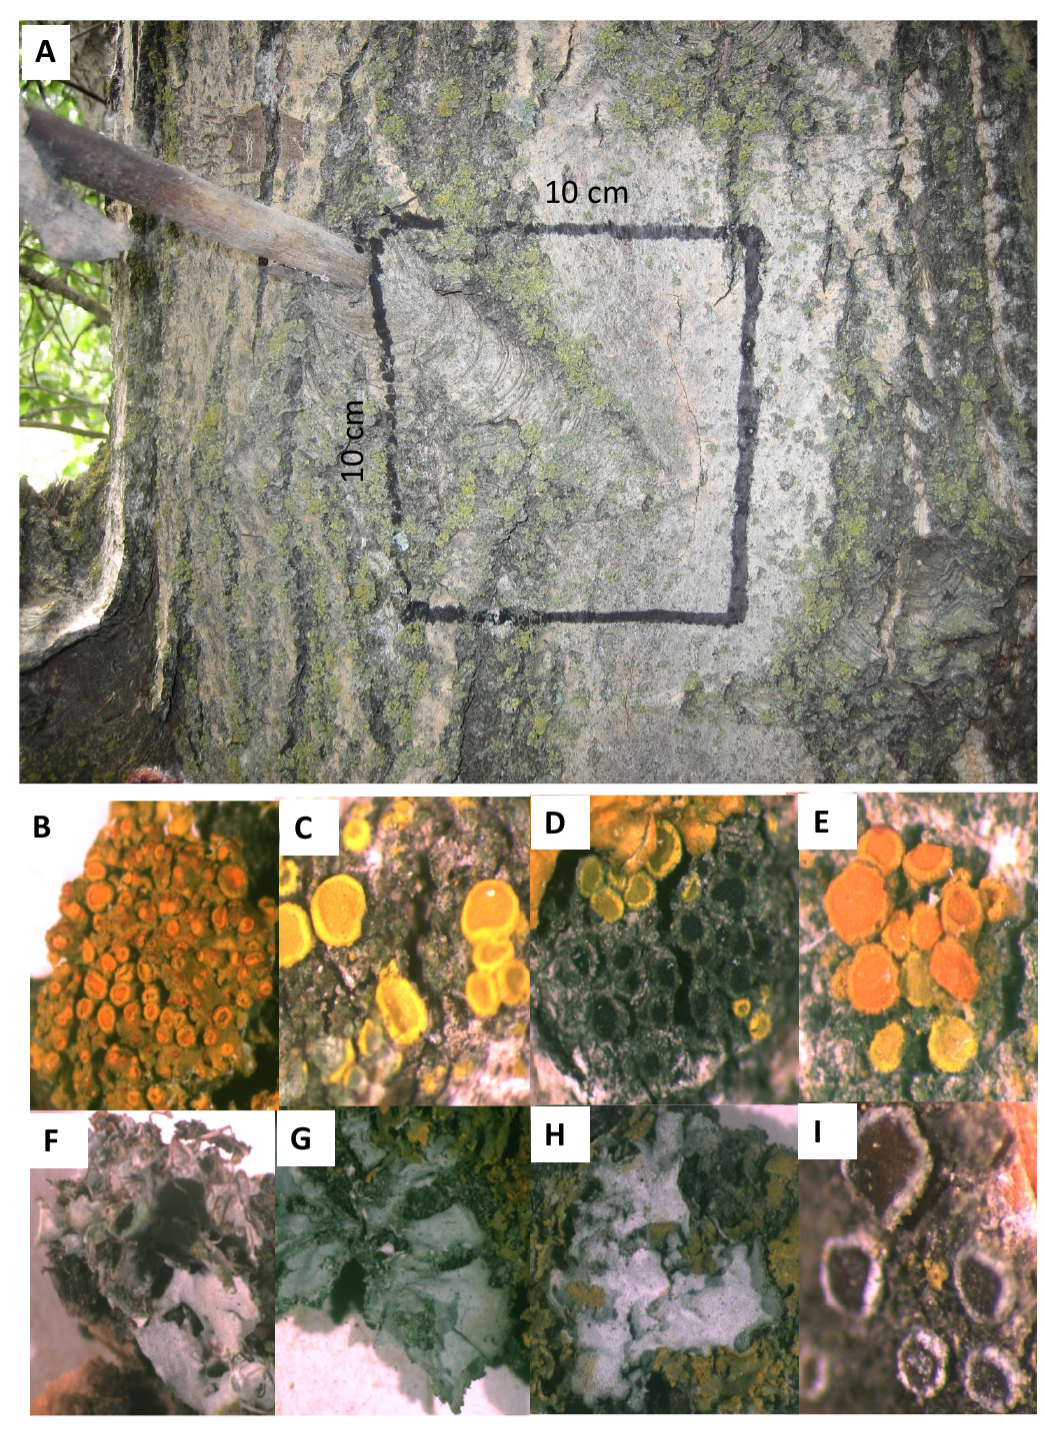
\includegraphics[width=\linewidth]{lcn_sampling.pdf}
\caption{The communities of bark lichens were observed in a common
  garden of replicated genotypes of narrowleaf cottonwood trees
  (\textit{P. angustifolia}) at the Ogden Nature Center (Ogden,
  UT). Lichens were sampled within a fixed area (10 cm$^2$) on
  individual trees (A and B). (C) a photo of a typical community of
  bark lichen species interacting on the trunk of a cottonwood tree,
  including one of the more abundant species, \textit{Xanthomendoza
    galericulata}, in the center. (D-K) shows the other lichen species
  observed, respectively:  \textit{X. montana}, \textit{Candelariella
    subdeflexa}, \textit{Rinodina} sp., \textit{Caloplaca holocarpa},
  \textit{Physcia adscendens}, \textit{Phyciella melanchra},
  \textit{Physcia undulata} and \textit{Lecanora hagenii}. Photo
  Credits: L.J. Lamit (A-C) and R.R. Naesbourg (D-K).}
\label{fig:lichen_sampling}
\end{figure}


\subsection*{Lichen Network Modeling and Analysis}

\textbf{LJL: This seems like a key point, one that really makes the
  study above and beyond.  I would make it clear with the phrasing
  that individual networks were created for each individual tree
  sampled, in this way we had replicated networks for each tree
  genotypes.}

We used the observations of lichens in the 1 cm$^2$ cells on individual
trees of \textit{P. angustifolia}. Unipartite networks were generated
using the conditional probabilities of each species pair, i.e. the
probability of observing one species given an observation of another
species $P(S_i | S_j)$, based on the method developed by
\citep{Araujo2011}. To calculate conditional probabilities, we
quantified the individual probabilities of species occurrences
$P(S_i)$ and the joint probability of co-occurrences $P(S_i,S_j)$
using the frequencies of each species and their co-occurrences. We
were then able to calculate the conditional probabilities of each
species pair as $P(S_i|S_j) = \frac{P(S_i,S_j)}{P(S_j)}$, based on the
axioms of probability. This yielded a matrix that could possibly be
asymetric, i.e. $P(S_i|S_j)$ does not have to be equal to
$P(S_j|S_i)$. Another important property of this matrix is that the
diagonal ($S_{ii}$) was equal to one for all species present and zero
for species that were not observed in any cell.

\textbf{MKL: regarding Lamit's question about the symmetry, the point
  is that direction of the interaction matters. The effect of species
  A on B can be different from B on A. No the matrix is not
  necessarily triangular (triangular being that the matrix either
  above or below the diagonal is completely zero).}

We then applied an analytical procedure to remove non-significant
links between species. This procedure determines if the joint
probability of a species pair (i.e. $P(S_i,S_j)$) is different from
zero (Fig.~\ref{fig:conet_method}).  Here, a confidence interval
$CI_{95\%}$ is calculated as as $CI_{95\%} = E[S_iS_j] * Z_{95\%} *
\sqrt{V(S_iS_j)}$, where the expected frequency of co-occurrences
E($S_iS_j$) is the total number of cells surveyed ($N$) times the
independent probabilities of each species $P(S_i) * P(S_j)$,
$Z_{95\%}$ is the Z-score for 95\% from a Z-distribution and the
expected variance of $E(S_iS_j)$ is the total number of cells times
the expected probability of $S_iS_j$ and its compliment
(i.e. $V(S_iS_j) = N * E[P(S_i,S_j)] * (1 - E[P(S_i,S_j)])$). If the
observed number of co-occurrence falls outside of the confidence
interval, the joint probability $P(S_i,S_j)$ is determined to be equal
to the product of the individual probabilities (i.e. $P(S_i) \dot
P(S_j)$), and the conditional probability reduces to the individual
probability of that species $P(S_i)$. Therefore, unless the
co-occurrence of a species pair falls outside the confidence interval,
the probability that the observation of one species given the other is
no different than simply observing that species alone. This enables us
to remove links from a given network by re-scaling the resulting
conditional probabilities by subtracting the individual probabilities
from the conditional probabilities (i.e. how different the conditional
probability is from the independent probability), which makes any
species with a non-significant conditional probability zero. The
resulting matrix ($\mathbf{D} = D_{ij}$) can be interpreted as how one
species impacts another with zero being no effect and values less than
or greater than zero interpreted as negative and positive effects,
respectively. Here, we will refer to this matrix ($\mathbf{D}$) as an
interaction matrix with the properties that it can be asymetric
(i.e. $P_{ij}$ does not necessarily equal $P_{ji}$), and the diagonal
($P_{ii}$) is zero (i.e. a species does not influence it's own
probability of being observed).

\textbf{LJL: This approach seems legit and it sound
  impressive. However, I admit that I think it is a bit above my head
  and possibly Tom’s, too. I have no doubt you did everything
  correct. But, it might be wise to get a friendly review from a mathy
  person just to be on the safe side. Perhaps Stuart in NC, or Aaron
  Ellison.} 

\textbf{MKL: agreed. This seems like a job for Bowker or Stuart. They
  can take a look on the next round of reviews.}

\begin{figure}[ht]
\centering
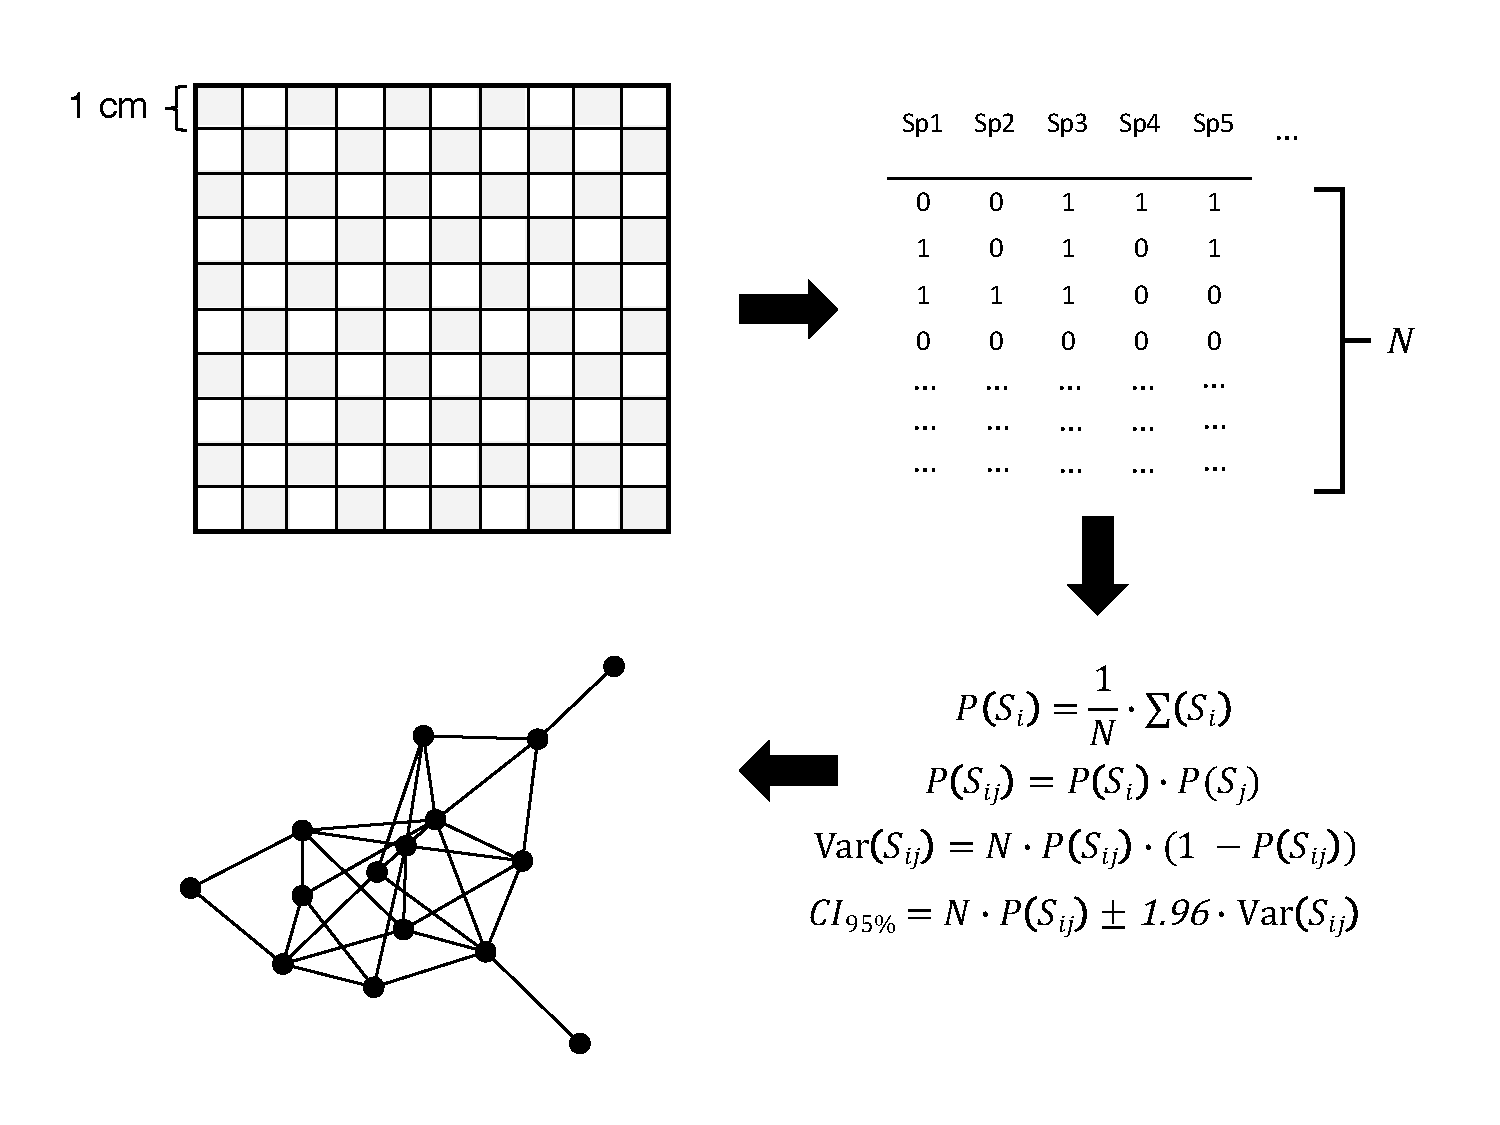
\includegraphics[width=\linewidth]{lcn_araujo_method.pdf}
\caption{Lichen interaction networks were constructed by conducting
  field observations in 1 cm$^2$ cells within a 10 cm$^2$ grid on each
  tree using a checkerboard pattern (grey cells). Thus, a set of $N$
  total cell observations were recorded for each tree with the
  presence or absence of each species recorded for each cell. Applying
  the probability-based network modeling method adapted from
  \cite{Araujo2011}, we calculated the conditional probabilities,
  $P(S_i|S_j)$, for all species pairs and removed (i.e. set equal to
  zero) species pairs whose joint probabilities, $P(S_i S_j)$, were
  not significant using a confidence interval based comparison of
  their observed co-occurrence frequency, $S_iS_j$, to that expected
  due to chance alone, $E[P(S_iS_j)] = P(S_i) P(S_j)$, and
  $P(S_i|S_j)$ reduces to $P(S_i)$, the observed individual
  probability of species $S_i$.}
\label{fig:conet_method}
\end{figure}


\textbf{LJL: I like the details here. THe one thing is that it sort of
  makes the reader think there is only one quadrat on a tree but
  infact there were two. I think you want to make sure to be explicit
  about the two. For analytical purposes, was all the data lumped so
  there was really functionally a 20cm by 10cm grid (just split into
  two pieces). Or, was the network made for each of the two grids and
  them averaged or combined in some way? My understanding is that it
  was more the first than the latter.}

\textbf{MKL: Yeah, it was the latter. I'm using two quadrats lumped
  together. I'll add more text here to clarify that.}


\subsection*{Statistical Analyses, Software and Data}

We used a combination of parametric and non-parametric, permutation
based frequentist statistical analyses to test for the effects of
genetic variation on lichen communities and their interaction
networks. To assess the effect of genotype on univariate responses, we
used additive, random effects models with Restricted Maximum
Likelihood (REML). We used a combination of Least Squares Regression,
Analysis of Variance (ANOVA) and correlation tests to quantify and
test for the relationship among other variables. Bark roughness,
lichen cover and species richness were square-root transformed to meet
the assumptions of homogeneity of variance and normality for these
tests.



For multivariate response variables, such as lichen community
composition and network structure, we used distance based multivariate
statistical approaches, including Permutational Analysis of Variance
(PerMANOVA) and Mantel tests. For all analyses, community composition
was relativized by species maxima to reduce the effect of the highly
abundant \textit{X. galericulata}. For community composition we used
Bray-Curtis dissimilarity, which has optimal performance with count
data \citep{Minchen1998}. To quantify the similarity of lichen
networks among individual trees, we calculated the pairwise Euclidean
distance of the $\mathbf{D}$ interaction matrices among all pairs of
trees.

For visualization of multivariate patterns, we used Non-metric
Multi-Dimensional Scaling (NMDS) \cite{ecodist} to produce
dimensionally reduced ordinations of these multi-variate responses and
fitted vectors for continuous predictor variables to the ordinated
values \cite{vegan}. Using random initial configurations with a
maximum of 500 iterations and a change in stress threshold of less
than 10$^{-12}$. Final configurations has the lowest stress with at
most a stress level of 0.10.


For each network, we also calculated two network metrics that measure
different structural aspects. We calculated the number of interactions
or ``links'' in each network, which provides a measure of the size of
the network \citep{Lau2015, Borrett2015}. We also calculated the
centralization of each network, which measures the evenness of the
distribution of interactions among the species in the network
\cite{Butts2005}. In a network with a low level of centralization
species have similar amount of interaction in the network, while a
network with a high level of centralization tends to one or small
subset of species that interact with other species. We used a related
function to calculate the centrality of each species in each network
as well. Although there are many other metrics, see \citep{Lau2017a},
we focus on a subset for the sake of simplicity and because some
metrics are not appropriate for our relatively small
communities. \textbf{In particular, we do not present analysis of the
  modularity (i.e. the degree of sub-grouping) because our community
  has relatively few species to form modules.} As with the other
response variables, the number of links was log-transformed and
centralization scores were square-root transformed to meet variance
and normality assumptions.

\textbf{LJL: I suggest deleting the highlighted part. And, just
  changing the sentence above it to “...because some metric (e.g.,
  modularity) are not appropriate...”  Too much emphasis on caviots
  will make some readers be uncertain. But, also, you can save some
  space that way.}

We have made all code and data available online. Code is available at
\url{github.com/communitygenetics/lcn}. Data is available via the
Harvard Dataverse (needs project ID). The project is also archived via
Zenodo at \url{zenodo.com/doiXXXXXX}. All analyses were conducted
using the programming language R version 3.4.2 (R Development Core
Team 2018).

\section*{Results}

%%% Results outline

%% Each of the ``%%'' correspond to paragraphs

%% Tree genotypes support distinct lichen networks
% fig:cn_onc
% table:onc_d_Ftable
% 1. Lichen network similarity permanova for genotype
%% geno     12   367.65 0.26937  2.3065   0.02860 *  
%% BR        1    23.63 0.01732  1.7792   0.18828    
%% pH        1     8.96 0.00656  0.6745   0.41866    
%% CN        1    37.70 0.02762  2.8379   0.08849 .  
%% CT        1    76.22 0.05585  5.7383   0.03310 *  
%% PC        1    28.50 0.02088  2.1458   0.14349    
%% SR        1   332.23 0.24342 25.0117 9.999e-05 ***
%% SE        1    51.59 0.03780  3.8843   0.04470 *  

% 2. C. subdeflexa was the most central species, primarily positive
% but tended to have a negative relationship with X. galariculata
% 0.73 +/- 0.14
% summary(aov(value ~ X2, data = melt(cen.spp)))
%%              Df Sum Sq Mean Sq F value Pr(>F)    
%% X2            8  27.04   3.380   8.086  3e-10 ***
%% Residuals   468 195.63   0.418                   

%% Network structural statistics varied among genotypes
% Fig: Total cover, richness and centrality among genotypes
% 1. Centrality genetically based (REML)
% 2. Number of linkages and modularity were not (REML)
% 3. Percent cover, richness genetically based, but evenness and
% diversity were not (REML)
% 4. Species richness correlated with network centrality, total cover
% was not (cor.test)

%% Genetically based tree traits correlated with network structure
% Fig:cn_chplot
% 1. Bark roughness but not tree chemistry (REML)
% 2. Bark roughness correlated with network similarity
% 3. Not correlated with species richness or centrality

%% Patterns were similar to wild stands
% Fig:
% 1. Network and trait correlations (PerMANOVA or MANTEL)
% 2. Community and network metric correlations (cor.test or lm)

%%% 

Networks were more similar as a result of having similar numbers of
interactions and distribution of interactions. The number of links
(PerMANOVA $R^2$ = 0.392, F 1 = 72.4348, $p$-value = 0.001) and
network centrality (PerMANOVA $R^2$ = 0.309, F 1 = 57.0440, $p$-value
= 0.001) were highly correlated with network similarity.  Tree
genotype significantly predicted network centrality (REML $R^2$ =
0.202, RLRT = 2.7801, $p$-value = 0.04012) but marginally predicted
the number of links (REML $R^2$ = 0.170, RLRT = 2.0484, $p$-value =
0.065) (Fig.~\ref{fig:cn_metrics}). Total cover was correlated with
the number of links (ANOVA $F_1$ = 6.867, $p$-value = 0.0114) and
centrality (ANOVA $F_1$ = 8.093, $p$-value = 0.0063). Lichen species
richness was also correlated with the number of links (ANOVA $F_1$ =
29.436, $p$-value = 0.000015) and centrality (ANOVA $F_1$ = 39.488,
$p$-value < 0.000001). Bark roughness, however, did not significantly
predict either the number of links (ANOVA $F_1$ = 2.897, $p$-value =
0.0946) or the centrality (ANOVA $F_1$ = 2.591, $p$-value = 0.1134) of
lichen networks (Supplementary Tables~\ref{tab:L_aov} and
~\ref{tab:cen_aov}).


\subsection{Some genetically based tree traits predicted lichen
  network structure}

Bark roughness predicted lichen communities. Percent rough bark varied
significantly among genotypes (REML $R^2$ = 0.378, RLRT = 10.69,
$p$-value = 0.0001), as did total lichen cover (REML $R^2$ = 0.172,
RLRT = 2.9627, $p$-value = 0.0375). However, lichen species richness
did not show a significant response to genotype (REML $R^2$ = 0.0981,
RLRT = 1.0001, $p$-value = 0.1366). Community composition was also
affected by tree genotype (PerMANOVA $R^2$ = 0.243, F 12 = 1.8221,
$p$-value = 0.0029). In addition, community composition was correlated
with bark roughness (PerMANOVA $R^2$ = 0.039, $F_1$ = 3.7408,
$p$-value = 0.0064), lichen cover (PerMANOVA $R^2$ = 0.342, $F_1$ =
32.8482, $p$-value = 0.0001) and lichen species richness (PerMANOVA
$R^2$ = 0.069, $F_1$ = 6.5958, $p$-value = 0.0002). However, after
controlling for the effect of tree genotype on community composition,
bark roughness did not significantly predict community composition
(PerMANOVA $R^2$ = 0.011, F 1 = 0.9938, $p$-value = 0.3841) but lichen
cover (PerMANOVA $R^2$ = 0.236, $F_1$ = 21.2661, $p$-value = 0.0001)
and lichen species richness (PerMANOVA $R^2$ = 0.054, $F_1$ = 4.9036,
$p$-value = 0.0011) were still significantly correlated with lichen
composition (Supplementary Tables~\ref{tab:com_ng_perm} and
~\ref{tab:rcom_perm}).


\subsection{Wild stand results}

\textbf{MKL: I removed the community similarity figure to simplify the
presentation of the results and improve the flow.}

%% \begin{figure}[ht]
%% \centering
%% 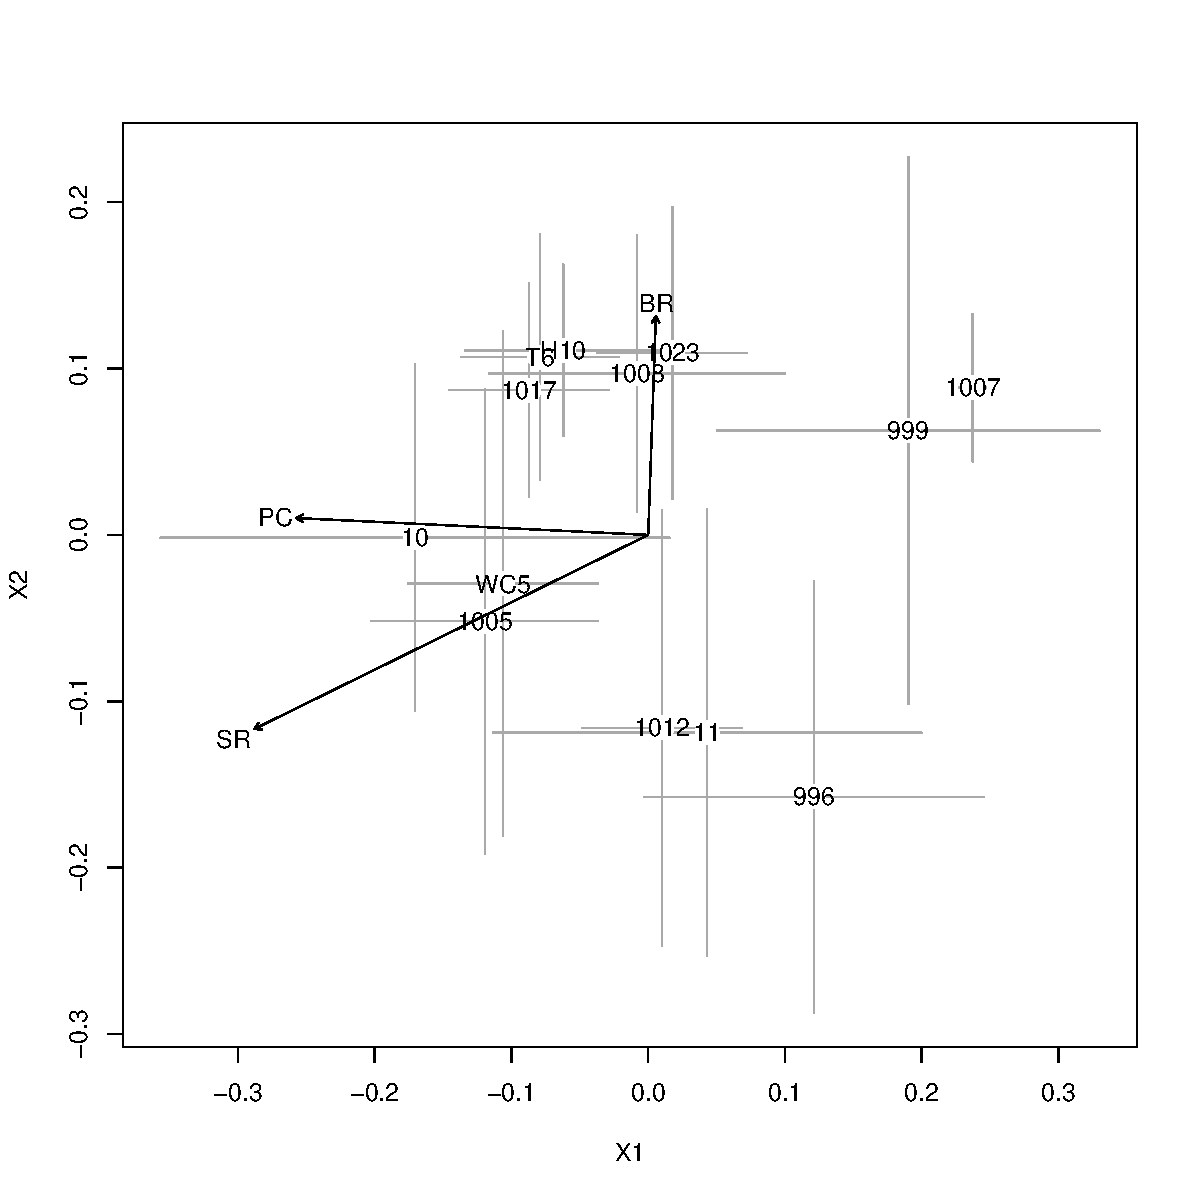
\includegraphics[width=\linewidth]{com_chplot_onc.pdf}
%% \caption{Lichen community composition varied among tree
%%   genotypes. Plot of the ordinated centroids ($\pm$ 1 S.E.) for the
%%   composition of lichen species (R$^2$ = 0.935, stress = 0.101) for
%%   each tree genotype (indicated by centroid labels). Centroids that
%%   are closer together have more similar lichen communities. Arrows
%%   show the direction and magnitude of correlation between bark
%%   roughness (BR), percent lichen colonization (PC) and lichen species
%%   richness (SR) and the ordinated community scores.x}
%% \label{fig:com_ch_plot}
%% \end{figure}

\textbf{LJL: Figure looks good. But, maybe making all lines a little
  thicker would look nicer and pop more.}

\textbf{LJL: Since we already published that tree genotypes differ in
  lichen composition, I wonder if we need to say somewhere in the
  manuscript why this test was run here. It seems to me it is
  important to verify this with a slightly different sampling method
  as used int eh 2015 paper, and for this specific set of
  genotypes. But, then does this test of composition just become
  something necessary just in a methodological variation that
  justifies the next step of examing network structure.  Something to
  think about. It might be that theNMDS should jsut go in a
  supplement, although I do like it here in some ways.  It might also
  be another approach to put the composition and other analyses after
  the network analysis results are presented. In this way, you could
  use the composition and results with vectors to help provide
  resolution on what is driving networks to differ among genotypes.}


\textbf{MKL: Adapt into a table.}


\textbf{TGW: clarify positive vs negative interactions.}

\begin{figure}[ht]
\centering
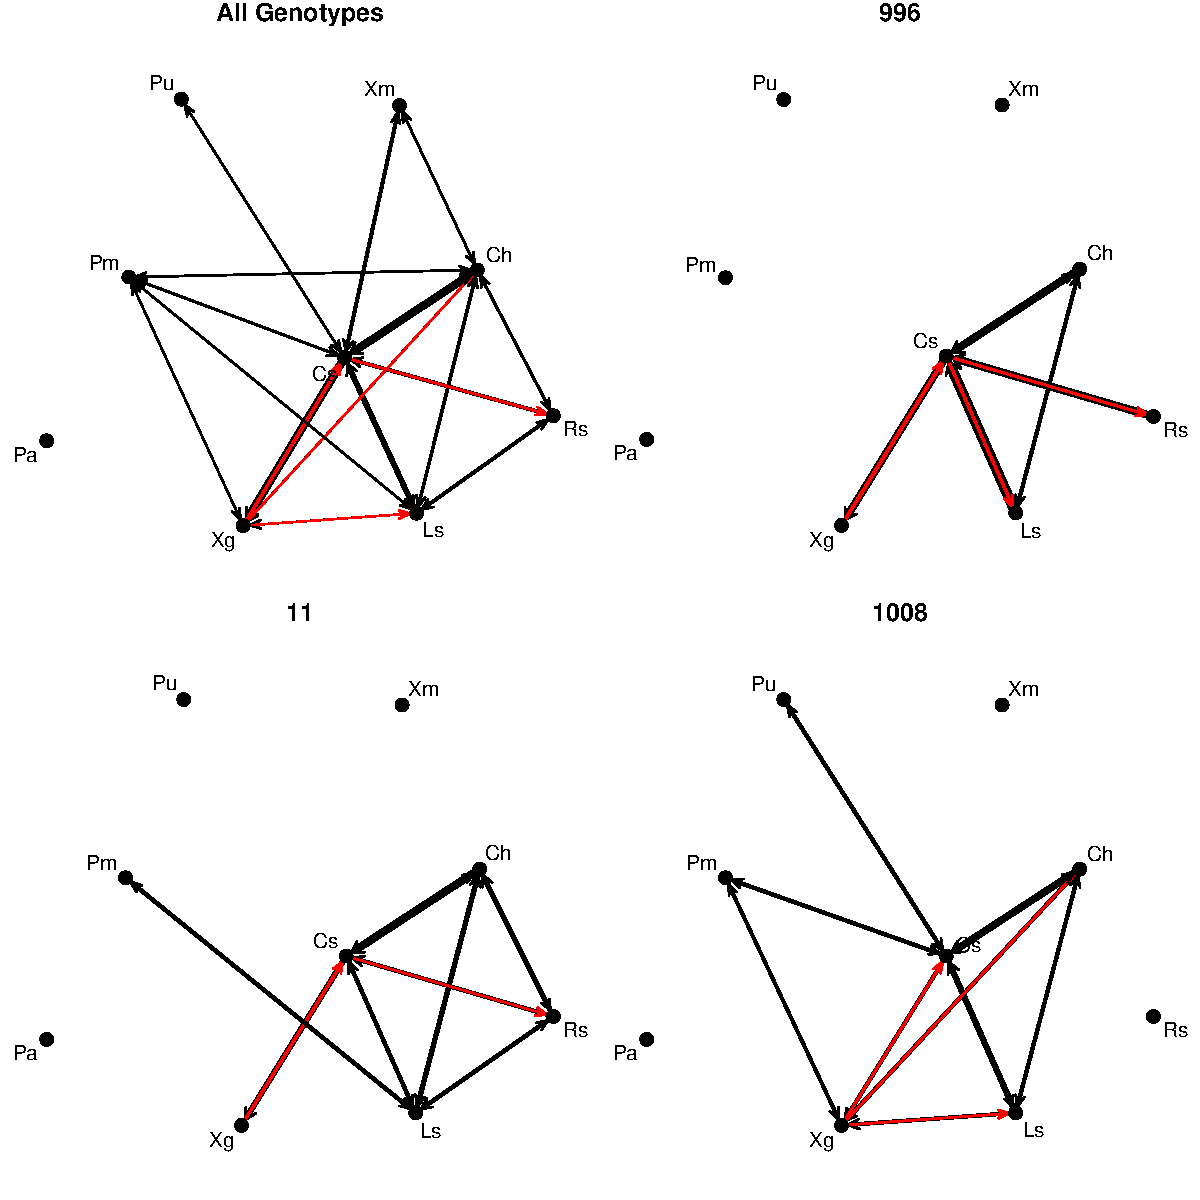
\includegraphics[width=\linewidth]{cn_onc.pdf}n
\caption{Lichen networks varied in structure among tree
  genotypes. Network diagrams of the mean lichen interaction matrices
  averaged for all trees and for several individual genotypes showing
  a range of interaction network structure. Directionality
  (arrowheads) and sign (red = negative, black = positive) of
  interactions are shown as edges between species (abbreviated by the
  first letter of the genus and specific epithet), which are scaled by
  their magnitude. The sign of the interaction is indicative of
  greater (positive) or lesser (negative) paired occurrences than
  expected relative to the overall frequency of occurrence of each
  species. Ecologically, the links in the network are likely the
  product of multiple types of interactions (e.g. mutualism,
  parasatism, competition, facilitation) that could vary over both
  space and time.}
\label{fig:geno_nets}
\end{figure}

\subsection{Tree genotypes support distinct lichen networks}

\textbf{MKL: Combine ~\ref{fig:geno_nets} and ~\ref{fig:cn_ch_plot}}

Lichen networks observed on trees of the same genotype tended to be
more similar. Tree genotype significantly predicted the similarity of
lichen interaction networks (PerMANOVA $R^2$ = 0.33795, F 12 = 2.5379,
$p$-value = 0.0050) (Fig.~\ref{fig:geno_nets} and
~\ref{fig:cn_ch_plot}). Bark roughness (PerMANOVA $R^2$ = 0.040, $F_1$
= 4.1680, $p$-value = 0.03770) and lichen species richness (PerMANOVA
$R^2$ = 0.424, $F_1$ = 44.5034, $p$-value = 9.999e-05) were
significant predictors of lichen network similarity, while total
lichen cover was a weak, marginally significant predictor (PerMANOVA
$R^2$ = 0.032, $F_1$ = 3.3573, $p$-value = 0.06779). However, after
controlling for the effect of tree genotype on lichen network
similarity, only species richness was a significant predictor of
lichen network similarity (PerMANOVA $R^2$ = 0.300, $F_1$ = 33.3755,
$p$-value = 0.00001), and neither bark roughness (PerMANOVA $R^2$ =
0.019, $F_1$ = 2.0858, $p$-value = 0.14699) nor lichen cover
(PerMANOVA $R^2$ = 0.019, $F_1$ = 2.1504, $p$-value = 0.14409) were
significant predictors (Supplementary Tables~\ref{tab:cn_ng_perm} and
~\ref{tab:cn_perm}). Community similarity was not correlated with
network similarity (Mantel Spearman $\rho$ = 0.092, $p$-value =
0.09500).

Networks were more similar as a result of having similar numbers of
interactions and distribution of interactions. The number of links
(PerMANOVA $R^2$ = 0.392, F 1 = 72.4348, $p$-value = 0.001) and
network centrality (PerMANOVA $R^2$ = 0.309, F 1 = 57.0440, $p$-value
= 0.001) were highly correlated with network similarity.  Tree
genotype significantly predicted network centrality (REML $R^2$ =
0.202, RLRT = 2.7801, $p$-value = 0.04012) but marginally predicted
the number of links (REML $R^2$ = 0.170, RLRT = 2.0484, $p$-value =
0.065) (Fig.~\ref{fig:cn_metrics}). Total cover was correlated with
the number of links (ANOVA $F_1$ = 6.867, $p$-value = 0.0114) and
centrality (ANOVA $F_1$ = 8.093, $p$-value = 0.0063). Lichen species
richness was also correlated with the number of links (ANOVA $F_1$ =
29.436, $p$-value = 0.000015) and centrality (ANOVA $F_1$ = 39.488,
$p$-value < 0.000001). Bark roughness, however, did not significantly
predict either the number of links (ANOVA $F_1$ = 2.897, $p$-value =
0.0946) or the centrality (ANOVA $F_1$ = 2.591, $p$-value = 0.1134) of
lichen networks (Supplementary Tables~\ref{tab:L_aov} and
~\ref{tab:cen_aov}).


\subsection{Some genetically based tree traits predicted lichen
  network structure}

Bark roughness predicted lichen communities. Percent rough bark varied
significantly among genotypes (REML $R^2$ = 0.378, RLRT = 10.69,
$p$-value = 0.0001), as did total lichen cover (REML $R^2$ = 0.172,
RLRT = 2.9627, $p$-value = 0.0375). However, lichen species richness
did not show a significant response to genotype (REML $R^2$ = 0.0981,
RLRT = 1.0001, $p$-value = 0.1366). Community composition was also
affected by tree genotype (PerMANOVA $R^2$ = 0.243, F 12 = 1.8221,
$p$-value = 0.0029). In addition, community composition was correlated
with bark roughness (PerMANOVA $R^2$ = 0.039, $F_1$ = 3.7408,
$p$-value = 0.0064), lichen cover (PerMANOVA $R^2$ = 0.342, $F_1$ =
32.8482, $p$-value = 0.0001) and lichen species richness (PerMANOVA
$R^2$ = 0.069, $F_1$ = 6.5958, $p$-value = 0.0002). However, after
controlling for the effect of tree genotype on community composition,
bark roughness did not significantly predict community composition
(PerMANOVA $R^2$ = 0.011, F 1 = 0.9938, $p$-value = 0.3841) but lichen
cover (PerMANOVA $R^2$ = 0.236, $F_1$ = 21.2661, $p$-value = 0.0001)
and lichen species richness (PerMANOVA $R^2$ = 0.054, $F_1$ = 4.9036,
$p$-value = 0.0011) were still significantly correlated with lichen
composition (Supplementary Tables~\ref{tab:com_ng_perm} and
~\ref{tab:rcom_perm}).


\subsection{Wild stand results}

\textbf{MKL: lichen networks in wild stands displayed similar
  structural patterns. Is it worth adding the wild stand? This will
  requite adding methods, results and more discussion.}

\textbf{MKL: Add the network metrics as vectors. Also add the wild
  stand as a point of reference or add as a supplementary figure.}

\begin{figure}[ht]
\centering
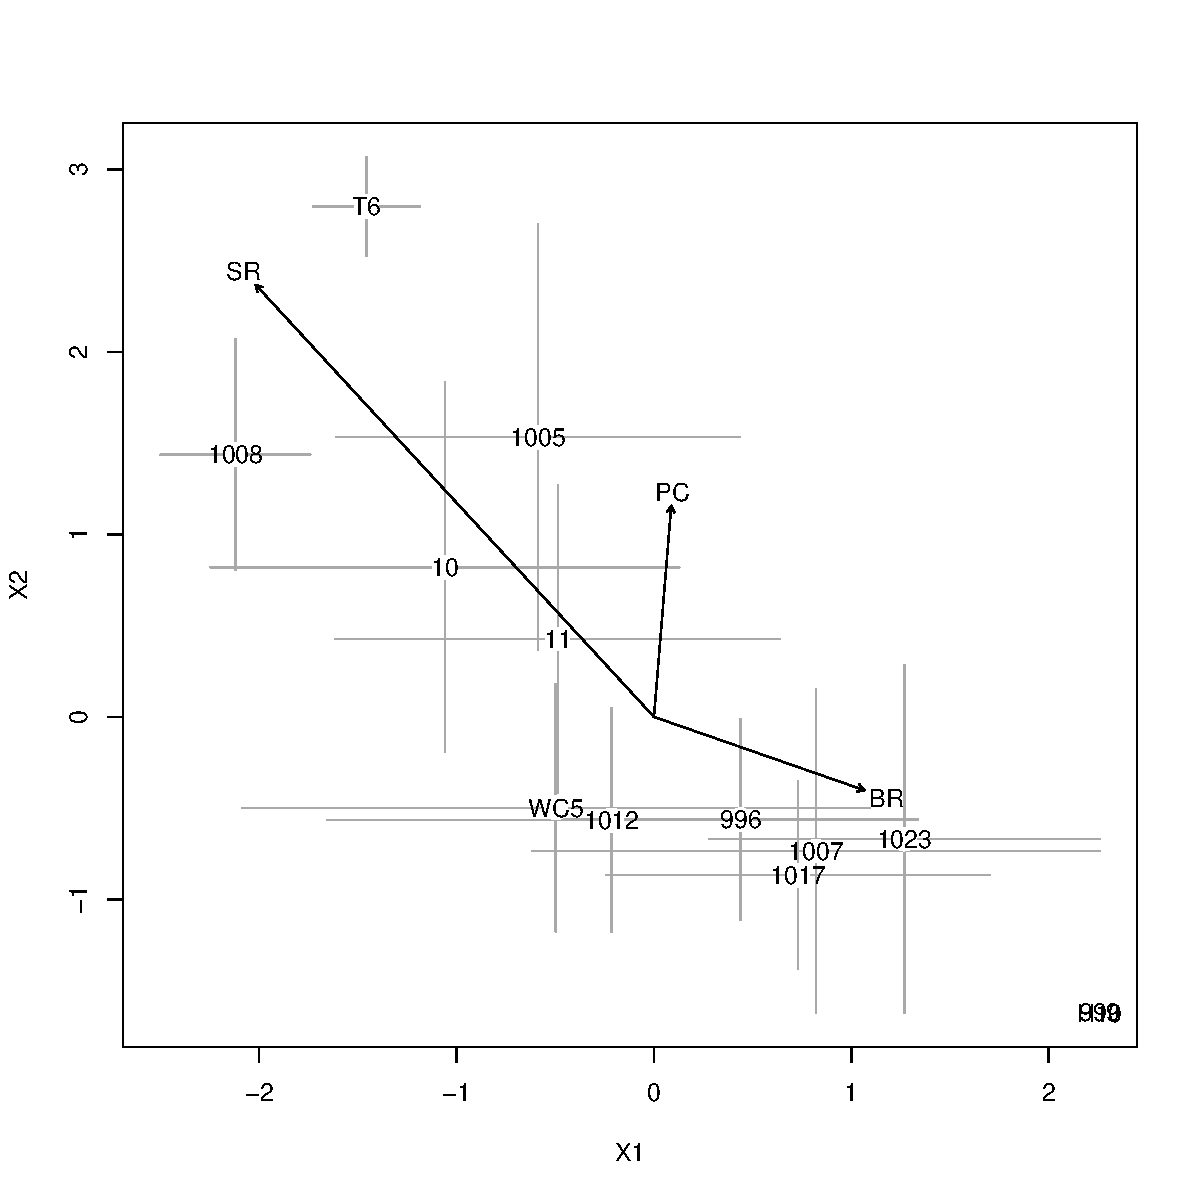
\includegraphics[width=\linewidth]{cn_chplot.pdf}
\caption{Significant lichen interaction network structure resulting
  from tree genotypic variation was observed in the common garden.
  The plot shows genotype centroids of NMDS ordinated (R$^2$ = 0.999,
  stress = 0.011) lichen networks ($\pm$ 1 S.E.). Centroids that are
  closer are more similar in the structure of their lichen
  networks. Arrows show the magnitude and direction of correlation of
  the ordinated networks with tree bark roughness (BR), percent cover
  of lichens (PC) and lichen species richness (SR).}
\label{fig:cn_ch_plot}
\end{figure}

\textbf{MKL: Need to re-organize the flow of the results.}


\textbf{LJL: It seems to me that the first two sentences here are the
  most important of the results. How can you make them stand out more?
  Maybe also they should go at the begining of the previous paragrpah,
  and then move that paragraph to being the first in the REsults
  section.}

\textbf{TGW: Here and in earlier paragraphs, a lot of stats are
  presented some of which are significant and some not.  For your
  topic sentence to be accepted, it seems readers need to know how
  many of the stats need to confirm the pattern and how many would it
  take to reject.  This paragraph has about 8 stats so need some
  overarching statement(s).  E.g., 7 of 8 analyses support our
  overarching hypothesis that ...  Same goes for other such paragraphs
  such as the 1st and last paras of the Results.}



\begin{figure}[ht]
\centering
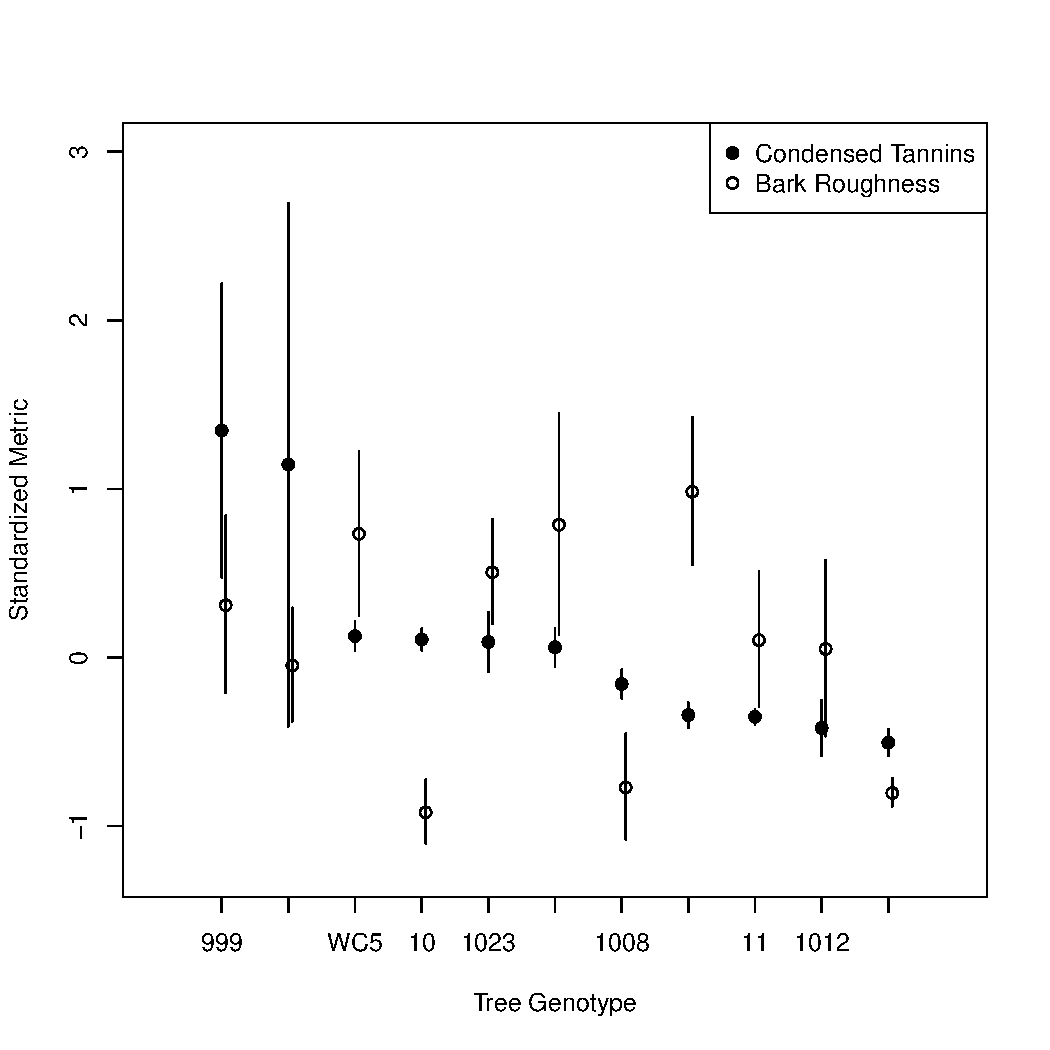
\includegraphics[width=\linewidth]{cn_metrics.pdf}
\caption{The impact of tree genotype on lichen network structure was
  indicative of variation in both the number variation in lichen
  interactions among species. Plot showing the means ($\pm$ 1 S.E.)
  for lichen network metrics, number of links and centralization, for
  each genotype. Both metrics are presented as standardized scores
  ($\frac{x - \bar{x}}{\sigma}$).}
\label{fig:cn_metrics}
\end{figure}



%% % latex table generated in R 3.5.1 by xtable 1.8-3 package
%% % Thu Jan 17 20:13:56 2019
%% \begin{table}[ht]
%% \centering
%% \begin{tabular}{llll}
%%   \hline
%% Response & H2 & $R^2$ & $p$-value \\ 
%%   \hline
%%   Percent Rough Bark           & 0.37835 & 0.37835 & 4e-04 \\ 
%%   Lichen Network               & 0.2784  & 0.3413  & 0.0074 \\ 
%%   Percent Lichen Cover         & 0.17279 & 0.17279 & 0.0362 \\ 
%%   Number of Network Links      & 0.16892 & 0.16892 & 0.0689 \\ 
%%   Network Centrality           & 0.17248 & 0.17248 & 0.0627 \\ 
%%   Lichen Community Composition & 0.08526 & 0.27703 & 0.09529 \\ 
%%   Network Modularity           & 0.04511 & 0.04511 & 0.2941 \\ 
%%   Lichen Species Richness      & 0.03578 & 0.03578 & 0.3137 \\ 
%%    \hline
%% \end{tabular}
%% \caption{Genotypic effects of cottonwood trees on the associated lichen community.} 
%% \label{tab:h2_table}
%% \end{table}

%% Supplementary: Stats tables


%% Not sure if these results should be included, it might be enough to
%% just tell the unipartite network story.
%% \subsection*{Genotypic variation increases stand-level lichen network modularity}
%% \begin{itemize}
%% \item Lichens displayed significant bipartite network structure
%% \item Bipartite network structure was greater than compared to the
%%   modularity based on a null model that randomizes with respect to genotype
%% \item z = 856.05271, $p$-value <= 0.00100 
%% \end{itemize}


%% In addition to including your tables within this manuscript file, PNAS
%% requires that each table be uploaded to the submission separately as a
%% “Table” file.  Please ensure that each table .tex file contains a
%% preamble, the \verb|\begin{document}| command, and the
%% \verb|\end{document}| command. This is necessary so that the
%% submission system can convert each file to PDF.



%% \begin{figure}
%% \centering
%% 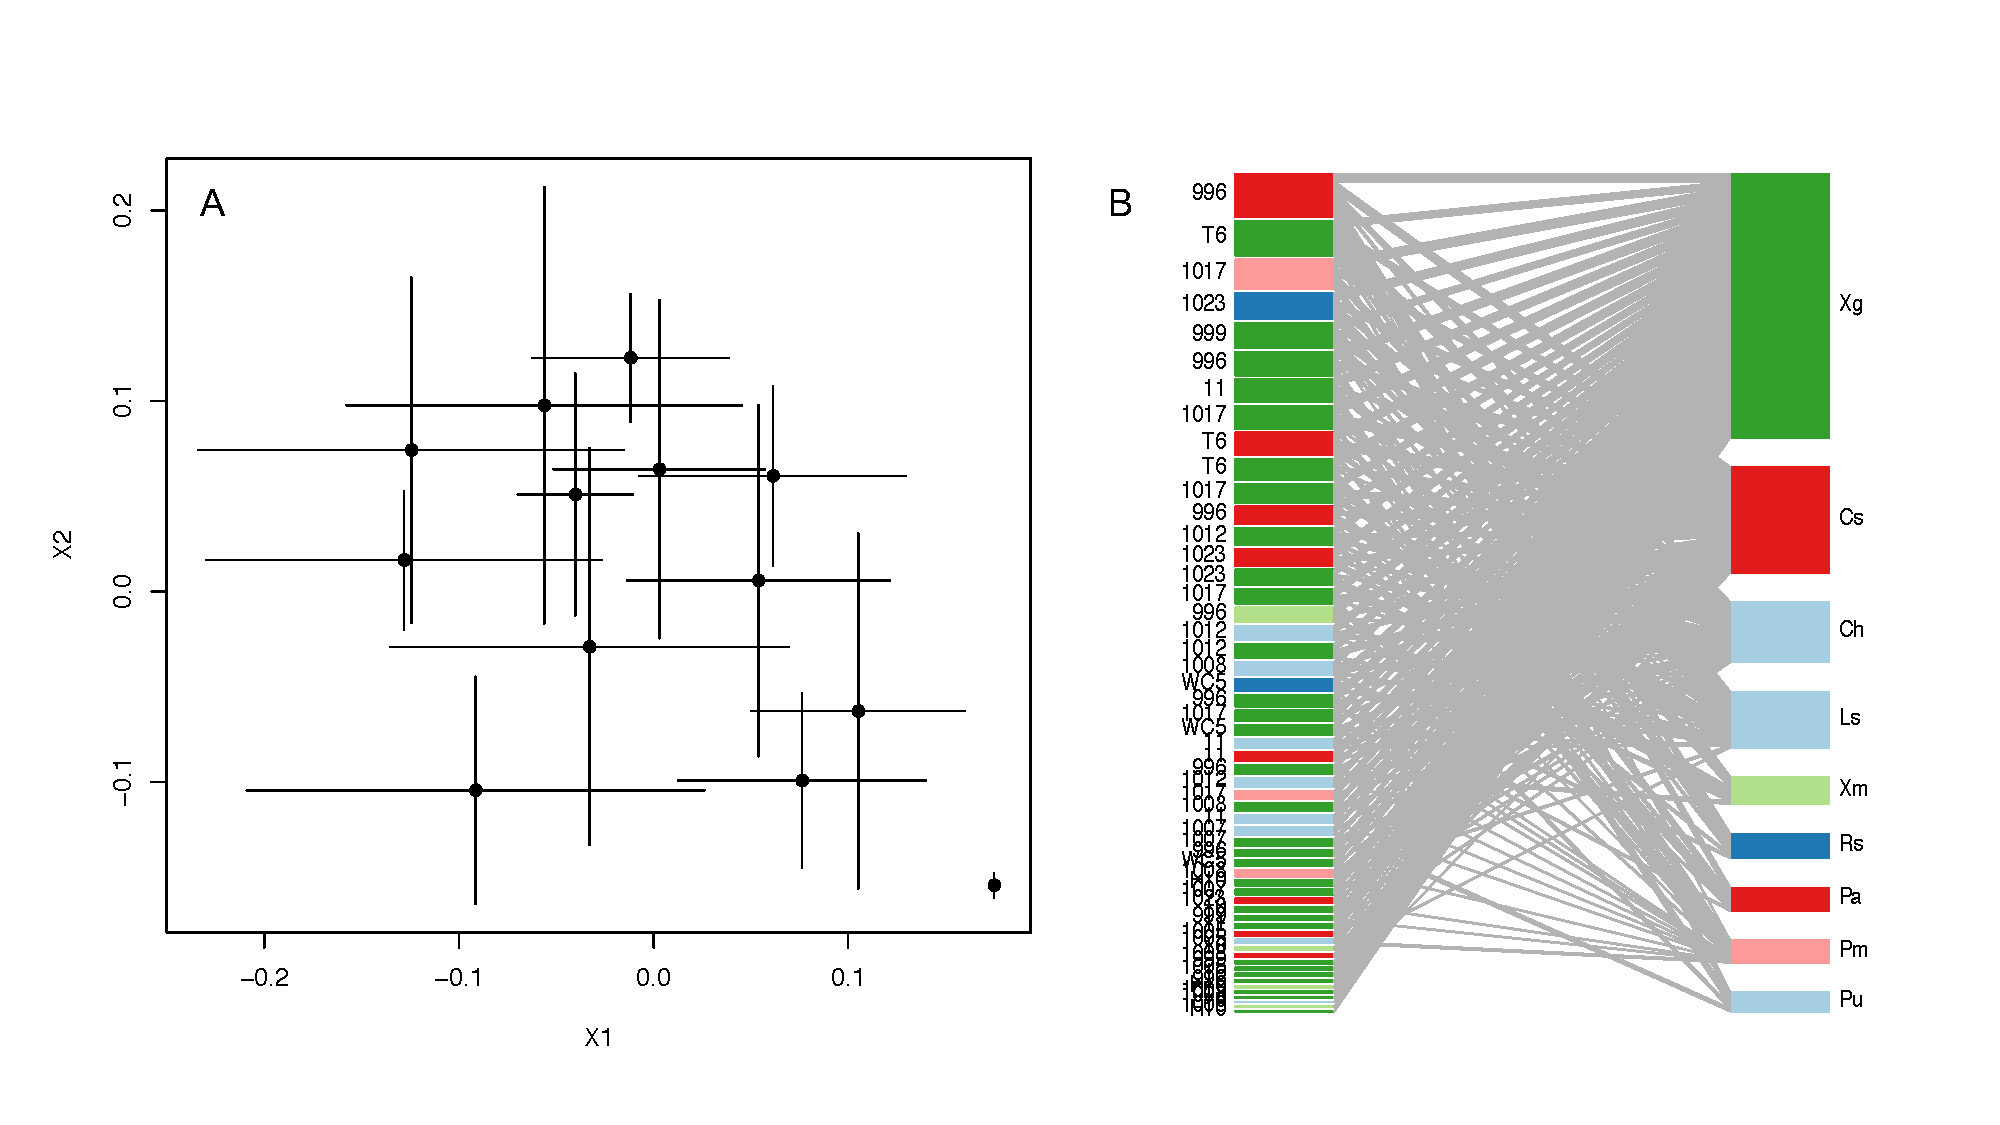
\includegraphics[width = \textwidth]{lcn_com_bpnet.pdf}
%% %% 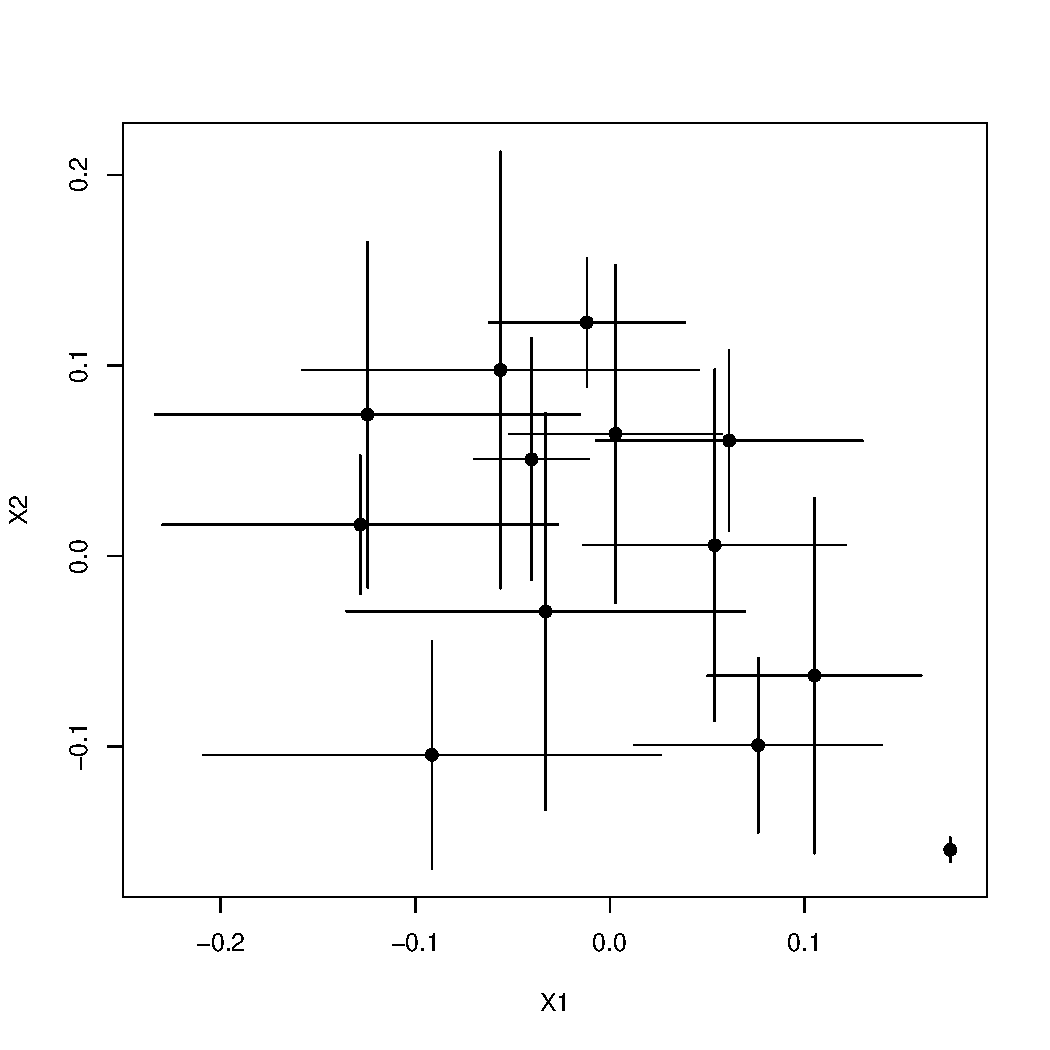
\includegraphics[width = 0.4\textwidth]{chp_com_onc.pdf}
%% %% 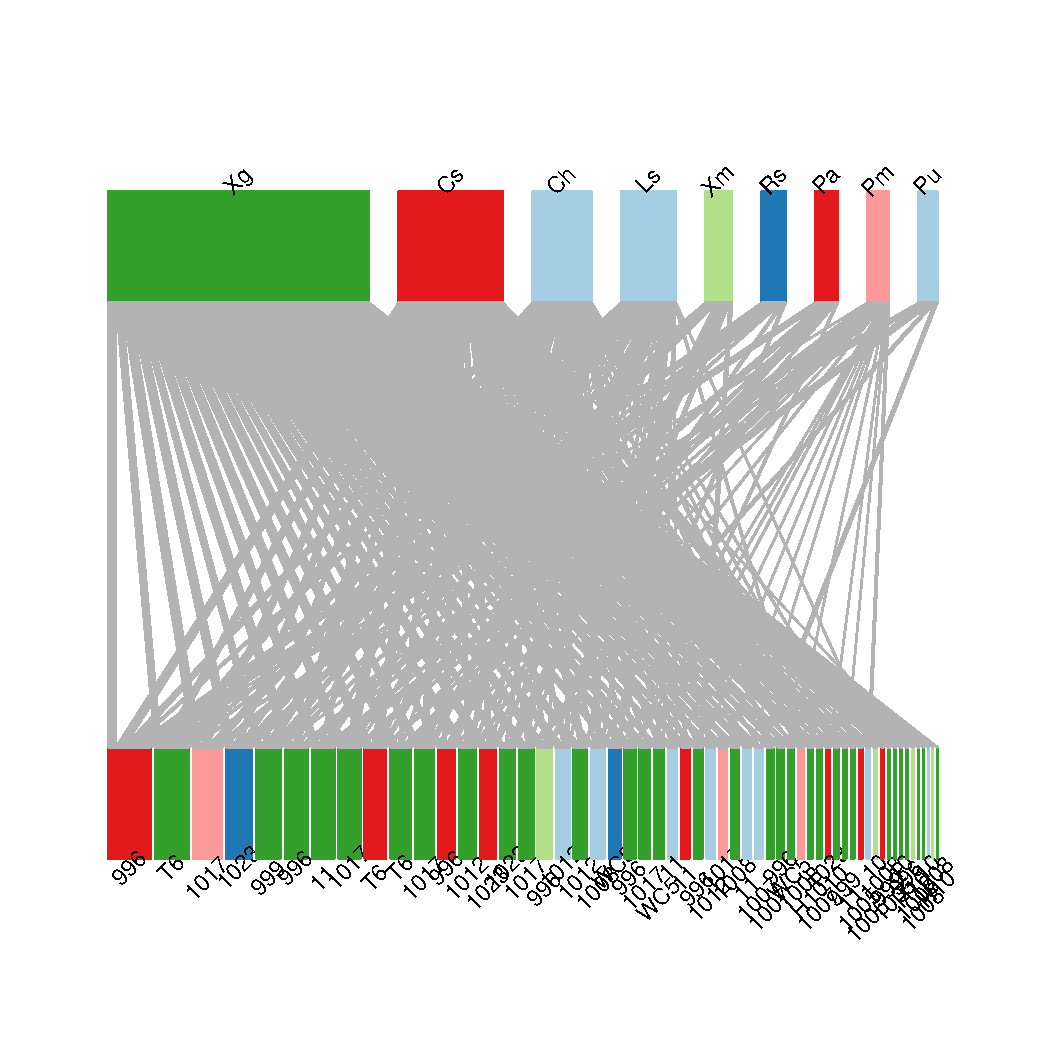
\includegraphics[width = 0.4\textwidth, angle = -90]{bp_net_onc.pdf}
%% \caption{Tree genotype variation in lichen community composition also
%%   contributed to genotype-species bipartite interaction network
%%   structure at the scale of the common garden stand. A) Plot of the
%%   ordinated community composition scores shown as centroids ($\pm$ 1
%%   S.E.). B) Bipartite interaction network based on the occurrences of
%%   lichen on individual cottonwood trees in the common garden. Edges
%%   connecting trees to lichen are scaled by the relative abundance of
%%   lichen. Nodes of lichen and trees are colored by their module
%%   membership.}
%% \label{fig:bpnet}
%% \end{figure}




}


\showmatmethods{} % Display the Materials and Methods section


\section*{Discussion}

%%% Discussion points

- Genotypic variation can lead to network variation
- Network structure is linked to function and dynamics. E.g. stability
- Community level selection may be possible, but this is not a
necessary factor for evolutionary dynamics to be relevant to ecological networks
- What are the conditions in which genetically based ecological network structure could have an effect?
- Network structure serves to amplify the signal of genetics


\textbf{TGW: I think window is too vague and this topic sentence needs
  to be much stronger for a journal like PNAS.  Might be stronger by
  saying "Our findings argue there is a genetic component to network
  structure, which implies that network structure could be subject to
  selection and networks can evolve."}

\textbf{TGW: Could we also make the comparsion that genetically more
  similar trees also have more similar communities?  We've done this
  in the past and it has worked, e.g., Randy's genetic similarity
  rule.}

\begin{itemize}
\item Genetic assembly rule = similar genetics will have more similar
  communities
\item What we don't know is whether or not these interactions will
  also lead to similar interactions among other species.
\item Thus, it would be possible for genetics to not only influence
  other species directly, but also indirectly by influencing the
  interactions among other species.
\end{itemize}

We observed significant lichen interaction structure that varied among
genotypes of a foundation tree species, narrowleaf cottonwood
(\textit{P. angustifolia}). We found that a genetically based trait,
bark roughness, partially explained the variation in lichen
interaction networks. Some of this variation in lichen networks was
related to both the overall abundance and species richness of lichen;
though, statistically controlling for the effect of genotype on these
variables indicates that a significant portion of the variance in
lichen species richness is due to a factor other than tree
genotype. By using network metrics, we were also able to probe for
specific characteristics of how these networks were responding to tree
genotype. We found that both number of links and the centralization of
the networks were highly correlated with network similarity and that
tree genotype significantly predicted network centrality but only
marginally predicted the number of network links. This latter result
could be due to the relationship between species richness and the
number of links in the network, which were significanlty correlated
with each other. We also found that bark roughness did not
significantly predict either the number of links or the centrality of
lichen networks, suggesting that bark roughness has some other effect
on the structure of the lichen networks. Taken together, these
findings support the hypothesis that genotypic variation in a
foundation species contributes to the structure of a network of
interacting species.

\textbf{LJL: 
I wonder if you need to have so much on richness here. 

Overall, I think you want to focus on the network reponses and
patterns among genotype first, and then go into mechanism later. I
think we don’t quite have a good mechanism yet so I don’t think it
needs to come up in the first paragrpah of the discussion.}



These findings point to the importance of understanding the community
level effects of genetic variation in plant functional traits and
highlights the potential for indirect effects of genetic variation to
propagate through networks of interacting species and trophic levels.

This work corroborates previous findings of the importance of plant
genetics in shaping community structure and ecosystem
processes. \citep{Bangert2008}


Altering the structure of interaction networks
presents a means for genetic effects to be magnified within the system
of interacting species. For example, \citep{Keith2017} showed that the
genetics based interactions of aphid resistant and aphid susceptible
trees resulted in different interaction networks of their associated
arthropod communities composed of 139 species. At the scale of
ecosystems, trophic networks or food webs direct and control the rates
of energy and nutrient flux \cite{Borgatti2006}. Furthermore, in a
predator-prey-plant study, Smith \cite{Smith2011}, showed that the
interactions among species across trophic levels depended on plant
genotype.

\textbf{LJL:  
It could be useful to point out that our findings are
  not related to trophic interactions, which is pretty cool.

Also,we talk about interaction networks but it is not clear to me if
the interactions tend to be positive or negative. Can we get at that
with the approach used? }


\textbf{TGW:  Is there any adaptive component to the tree in having
  certain lichen communities?  e.g., can they feed back to affect tree
  performance in some way or is this a passive outcome of a trait that
  affects bark for other adaptive reasons and lichens are passive
  players that tag along for the ride?  I could envision that lichens
  covering the bark of a tree act as a barrier between insects and
  pathogens, much like ectomycorrhizae cover fine roots as a first
  line of defense by invading microorganisms.  Uptake of N that gets
  passed to the tree??}


\textbf{TGW: might be good to cite papers on competition in lichens or
  other organizing factors to back up the least expected statement.
  as epiphytes we might not expect them to care.}

\textbf{TGW: I think we need to emphasize the long-term nature of our
  common garden study as very few common garden studies of lichens
  likely exist. Any refs on this? If true might want to mention this
  up front in intro.}

\textbf{MKL: Environmental filtering is evidenced by species richness,
  but also possibly species interaction varying based on environment
  as networks varied in terms of sign and magnitude as well.}

\textbf{MKL: The effect of bark roughness on network similarity was
  primarily genetically based, and there are likely other factors at
  play.}

\textbf{Discussion of network implications for stability with genetics.}

Although our study was conducted with a community of lichens, these
results should be generalized to other groups of diverse organisms
around the world that also exhibit significant genetic signals at the
community level \cite{Rowntree2011, Whitham2012}. In the face of the
high degree of complexity and potential context dependency of
ecological processes, the current study points to the utility of
considering the spatial and temporal scales of interactions, as
discussed to some in previous studies \cite{Bangert2006, Zook2010,
  Zytynska2012}. In the present study, we found that community
assembly processes, such as environmental filtering and species
interactions, are genetically based. This is likely due, in part, to
the large difference in the differences in size and longevity of the
lichen and cottonwood individuals with the trees determining the
environment in which the lichen occur. We suggest that future work
would be aided by determining these modules within the biotic
community that include species with similar differences in body-size
and time-scales. As heritable variation is the raw material for
natural selection to act upon, a genetic basis for interaction network
structure indicates evolutionary dynamics should be considered at the
community level and that conserving genetic variation is important to
consider in efforts to restore or preserve complex species
interactions and their associated ecosystem functions
\cite{Evans2013}.  With such findings, it appears that we are closer
to understanding the evolutionary drivers of Darwin's entangled bank
and the interconnectedness of species in complex communities.


%% Please include your acknowledgments here, set in a single
%% paragraph. Please do not include any acknowledgments in the
%% Supporting Information, or anywhere else in the manuscript.

\acknow{This work was supported by the National Science Foundation grant
(DEB-0425908) and Integrative Graduate Research Traineeship (IGERT)
fellowships for M.L. and L.L. The Ogden Nature Center staff helped to
maintain the common gardens. Lichen sampling was supported by Todd
Wojtowicz, Luke Evans and David Solance Smith.}

\showacknow{} % Display the acknowledgments section

\bibliography{lichen_network_genetics}

\newpage

\section*{Supplementary Materials}

\textbf{TGW: I know you commented about not talking about H2 in the
  text, but since you have the data, why not?  All heritability
  findings only apply for the environment or common garden they were
  measured in as does the rest of the findings presented in this
  paper.}

% latex table generated in R 3.4.4 by xtable 1.8-2 package
% Tue Nov 13 15:56:44 2018
\begin{table}[ht]
\centering
\begin{tabular}{llll}
  \hline
Response & Predictor & p-value & H2 \\ 
  \hline
Percent Lichen Cover & Tree Genotype & 0.0356 & 0.17 \\ 
  Lichen Species Richness & Tree Genotype & 0.1443 & 0.1 \\ 
  Percent Rough Bark & Tree Genotype & 8e-04 & 0.38 \\ 
  Lichen Network & Genotype & 0.0431 & 0.17 \\ 
  Number of Network Links & Genotype & 0.0796 & 0.15 \\ 
  Network Centrality & Genotype & 0.1351 & 0.12 \\ 
   &  &  &  \\ 
   &  &  &  \\ 
   &  &  &  \\ 
   \hline
\end{tabular}
\caption{Genotypic effects of cottonwood trees on the associated lichen community.} 
\label{tab:h2_table}
\end{table}
 

\setcounter{figure}{0}
\setcounter{table}{0}

\begin{figure}[ht]
\centering
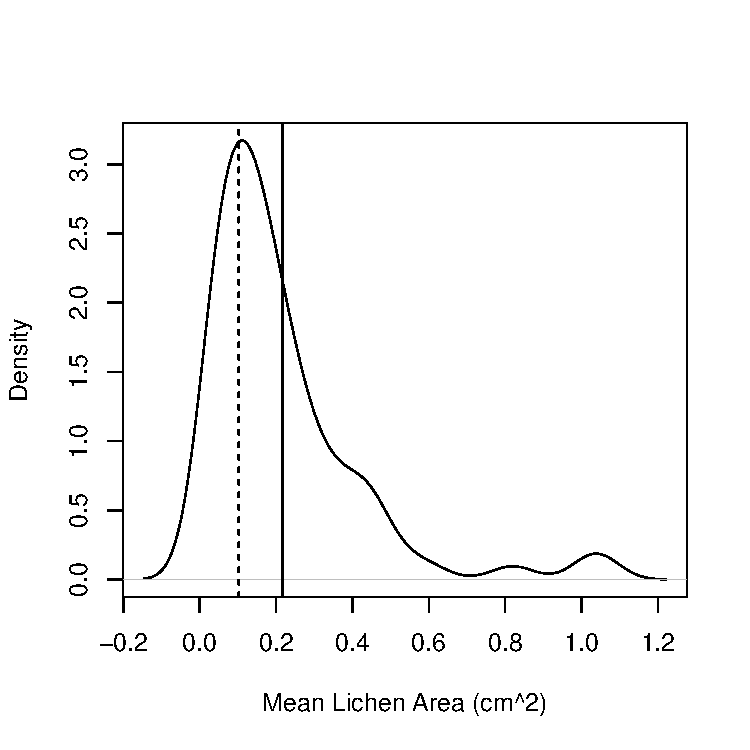
\includegraphics[width=\linewidth]{supplement/xg_size.pdf}
\caption{Density plot of the median lichen thallus area (cm$^2$). }
\label{fig:SI_xg_median}
\end{figure}

% latex table generated in R 3.5.2 by xtable 1.8-2 package
% Fri Mar  8 12:06:04 2019
\begin{table}[ht]
\centering
\begin{tabular}{lrrrrr}
  \hline
 & Df & SumOfSqs & R2 & F & Pr($>$F) \\ 
  \hline
BR & 1 & 0.44 & 0.04 & 3.74 & 0.0064 \\ 
  PC & 1 & 3.86 & 0.34 & 32.85 & 0.0001 \\ 
  SR & 1 & 0.78 & 0.07 & 6.60 & 0.0002 \\ 
  Residual & 53 & 6.23 & 0.55 &  &  \\ 
  Total & 56 & 11.31 & 1.00 &  &  \\ 
   \hline
\end{tabular}
\caption{PerMANOVA Pseudo-F Table showing the predictors of community similarity.} 
\label{tab:com_ng_perm}
\end{table}
 
% latex table generated in R 3.5.2 by xtable 1.8-2 package
% Fri Mar  8 12:06:04 2019
\begin{table}[ht]
\centering
\begin{tabular}{lrrrrr}
  \hline
 & Df & SumOfSqs & R2 & F & Pr($>$F) \\ 
  \hline
geno & 12 & 2.75 & 0.24 & 1.82 & 0.0029 \\ 
  BR & 1 & 0.12 & 0.01 & 0.99 & 0.3841 \\ 
  PC & 1 & 2.67 & 0.24 & 21.27 & 0.0001 \\ 
  SR & 1 & 0.62 & 0.05 & 4.90 & 0.0011 \\ 
  Residual & 41 & 5.15 & 0.46 &  &  \\ 
  Total & 56 & 11.31 & 1.00 &  &  \\ 
   \hline
\end{tabular}
\caption{PerMANOVA Pseudo-F Table showing the predictors of community similarity.} 
\label{tab:rcom_perm}
\end{table}
 
% latex table generated in R 3.5.2 by xtable 1.8-2 package
% Thu Jan 31 16:10:56 2019
\begin{table}[ht]
\centering
\begin{tabular}{lrrrrr}
  \hline
 & Df & SumOfSqs & R2 & F & Pr($>$F) \\ 
  \hline
BR & 1 & 61.42 & 0.04 & 4.17 & 0.0377 \\ 
  PC & 1 & 49.47 & 0.03 & 3.36 & 0.0678 \\ 
  SR & 1 & 655.76 & 0.42 & 44.50 & 0.0001 \\ 
  Residual & 53 & 780.96 & 0.50 &  &  \\ 
  Total & 56 & 1547.61 & 1.00 &  &  \\ 
   \hline
\end{tabular}
\caption{PerMANOVA Pseudo-F Table showing the predictors of network similarity.} 
\label{tab:cn_perm_ng}
\end{table}
 
% latex table generated in R 3.5.2 by xtable 1.8-2 package
% Thu Jan 31 16:10:56 2019
\begin{table}[ht]
\centering
\begin{tabular}{lrrrrr}
  \hline
 & Df & SumOfSqs & R2 & F & Pr($>$F) \\ 
  \hline
geno & 12 & 450.52 & 0.29 & 2.69 & 0.0094 \\ 
  BR & 1 & 29.11 & 0.02 & 2.09 & 0.1470 \\ 
  PC & 1 & 30.01 & 0.02 & 2.15 & 0.1441 \\ 
  SR & 1 & 465.78 & 0.30 & 33.38 & 0.0001 \\ 
  Residual & 41 & 572.18 & 0.37 &  &  \\ 
  Total & 56 & 1547.61 & 1.00 &  &  \\ 
   \hline
\end{tabular}
\caption{PerMANOVA Pseudo-F Table showing the predictors of network similarity.} 
\label{tab:cn_perm}
\end{table}
 
% latex table generated in R 3.5.2 by xtable 1.8-2 package
% Fri Mar  8 12:06:04 2019
\begin{table}[ht]
\centering
\begin{tabular}{lrrrrr}
  \hline
 & Df & Sum Sq & Mean Sq & F value & Pr($>$F) \\ 
  \hline
BR & 1 & 102.25 & 102.25 & 2.78 & 0.1016 \\ 
  PC & 1 & 239.57 & 239.57 & 6.50 & 0.0137 \\ 
  SR & 1 & 956.96 & 956.96 & 25.98 & 0.0000 \\ 
  Residuals & 53 & 1952.23 & 36.83 &  &  \\ 
   \hline
\end{tabular}
\caption{ANOVA F Table showing the predictors of the number of network links.} 
\label{tab:L_aov}
\end{table}
 
% latex table generated in R 3.5.2 by xtable 1.8-2 package
% Fri Mar  8 12:06:04 2019
\begin{table}[ht]
\centering
\begin{tabular}{lrrrrr}
  \hline
 & Df & Sum Sq & Mean Sq & F value & Pr($>$F) \\ 
  \hline
BR & 1 & 3.77 & 3.77 & 2.17 & 0.1463 \\ 
  PC & 1 & 6.46 & 6.46 & 3.72 & 0.0590 \\ 
  SR & 1 & 56.48 & 56.48 & 32.55 & 0.0000 \\ 
  Residuals & 53 & 91.95 & 1.73 &  &  \\ 
   \hline
\end{tabular}
\caption{ANOVA F Table showing the predictors of network centralization.} 
\label{tab:cen_aov}
\end{table}
 
% latex table generated in R 3.5.2 by xtable 1.8-2 package
% Fri Mar  8 12:06:04 2019
\begin{table}[ht]
\centering
\begin{tabular}{lrrrrr}
  \hline
 & Df & SumOfSqs & R2 & F & Pr($>$F) \\ 
  \hline
L & 1 & 1330.80 & 0.86 & 734.67 & 0.0010 \\ 
  Cen & 1 & 118.99 & 0.08 & 65.69 & 0.0010 \\ 
  Residual & 54 & 97.82 & 0.06 &  &  \\ 
  Total & 56 & 1547.61 & 1.00 &  &  \\ 
   \hline
\end{tabular}
\caption{PerMANOVA Pseudo-F Table showing the predictors of network similarity.} 
\label{tab:cn_L_cen_perm}
\end{table}
 


\end{document}

%% \subsection*{Supporting Information (SI)}

%% Authors should submit SI as a single separate PDF file, combining
%% all text, figures, tables, movie legends, and SI references.  PNAS
%% will publish SI uncomposed, as the authors have provided it.
%% Additional details can be found here:
%% \href{http://www.pnas.org/page/authors/journal-policies}{policy on
%% SI}.  For SI formatting instructions click
%% \href{https://www.pnascentral.org/cgi-bin/main.plex?form_type=display_auth_si_instructions}{here}.
%% The PNAS Overleaf SI template can be found
%% \href{https://www.overleaf.com/latex/templates/pnas-template-for-supplementary-information/wqfsfqwyjtsd}{here}.
%% Refer to the SI Appendix in the manuscript at an appropriate point
%% in the text. Number supporting figures and tables starting with S1,
%% S2, etc.

%% Authors who place detailed materials and methods in an SI Appendix
%% must provide sufficient detail in the main text methods to enable a
%% reader to follow the logic of the procedures and results and also
%% must reference the SI methods. If a paper is fundamentally a study
%% of a new method or technique, then the methods must be described
%% completely in the main text.

%% \subsubsection*{SI Datasets} 

%% Supply Excel (.xls), RTF, or PDF files. This file type will be
%% published in raw format and will not be edited or composed.

%% \subsubsection*{SI Movies}

%% Supply Audio Video Interleave (avi), Quicktime (mov), Windows Media
%% (wmv), animated GIF (gif), or MPEG files and submit a brief legend
%% for each movie in a Word or RTF file. All movies should be
%% submitted at the desired reproduction size and length. Movies
%% should be no more than 10 MB in size.


%% \subsubsection*{3D Figures}

%% Supply a composable U3D or PRC file so that it may be edited and
%% composed. Authors may submit a PDF file but please note it will be
%% published in raw format and will not be edited or composed.

